\documentclass[12pt,twoside,letterpaper]{memoir}

\usepackage{import}
%% GENERAL ADD ONS %%%%%%%%%%%%%%%%%%%%%%%%%%%%%%%%%%%%%%%%%%%%%%%%%%%%%%%%%%%%

\usepackage[dvipsnames]{xcolor}  %% Must come before Tikz etc.
\usepackage[many]{tcolorbox}
\usepackage{dcounter}
\usepackage{enumerate}
\usepackage{graphicx}
\usepackage[
    hyperindex=true,
    colorlinks=true,
    linkcolor=teal,
    citecolor=ForestGreen]{hyperref}
\usepackage{float}     %% given captions to listings and types.
\usepackage{caption}
\usepackage{subcaption}
% \usepackage{aeguill}  %% IF NEEDED INCLUDE IN Content.tex near top
\usepackage[light]{kpfonts} % Nice Adobe Font
\usepackage{pifont} % \xmark
    \newcommand{\cmark}{\ding{51}}%
    \newcommand{\xmark}{\ding{55}}%

%% TIKZ %%%%%%%%%%%%%%%%%%%%%%%%%%%%%%%%%%%%%%%%%%%%%%%%%%%%%%%%%%%%%%%%%%%%%%%
\usepackage{tikz}
\usepackage{tikz-cd}
    \usetikzlibrary{positioning,arrows,backgrounds}
%%%%%%%%%%%%%%%%%%%%%%%%%%%%%%%%%%%%%%%%%%%%%%%%%%%%%%%%%%%%%%%%%%%%%%%%%%%%%%%

%% MATH %%%%%%%%%%%%%%%%%%%%%%%%%%%%%%%%%%%%%%%%%%%%%%%%%%%%%%%%%%%%%%%%%%%%%%%

\usepackage{amsmath,amsthm,amssymb}

\newcommand{\bigforall}{\mbox{\Large $\mathsurround0pt\forall$}}
\newcommand{\bigexists}{\mbox{\Large $\mathsurround0pt\exists$}}


\usepackage{bussproofs}  %% proof diagrams
\usepackage{wasysym} % \Leftcircle
\usepackage{mathtools}  % left/right harpoons
% \usepackage{lscape}  %% Landscape pages.
% \usepackage{longtable}  %% tables that span 2 pages

%%%%%%%%%%%%%%%%%%%%%%%%%%%%%%%%%%%%%%%%%%%%%%%%%%%%%%%%%%%%%%%%%%%%%%%%%%%%%%%

\usepackage{pdfpages}
% \usepackage{zref-abspos} % Used to know where digress/focus starts/ends

%% STYLE CHAPTERS %%%%%%%%%%%%%%%%%%%%%%%%%%%%%%%%%%%%%%%%%%%%%%%%%%%%%%%%%%%%%
\makechapterstyle{invhangnum}{%
  \setlength\beforechapskip{0pt}%
  \renewcommand*\chapterheadstart{\vspace{\beforechapskip}}%
  \setlength\afterchapskip{2\onelineskip plus .2\onelineskip minus 0.2\onelineskip}%  
  \renewcommand\chaptitlefont{\Huge\bfseries}
  \setlength\midchapskip{-\baselineskip}%
  \renewcommand\chapnumfont{\Huge\bfseries}
  \renewcommand*{\printchaptername}{}
  \renewcommand*{\chapternamenum}{}
  \renewcommand*{\printchapternum}{%
      \raisebox{\dimexpr\midchapskip+\baselineskip\relax}[0pt][0pt]{%
        \makebox[0pt][l]{%
        \makebox[\dimexpr\textwidth+4em\relax][l]{%
          \parbox[t]{\textwidth}{\mbox{}}%
          \parbox[t]{4em}{\hfill\chapnumfont \thechapter}}}}}%
  \renewcommand*{\printchaptertitle}[1]{%
    \raisebox{\dimexpr\midchapskip+\baselineskip\relax}[0pt][0pt]{%
      \parbox[t]{\textwidth}{\raggedright\chaptitlefont ##1}}}%
}
\chapterstyle{invhangnum}
\newlength{\digresslen}
% \chapterstyle{hangnum}
% \hangsecnum

    \usepackage{eso-pic}   %% Used to add gray strip to side of pages.
    %%%%%%%%% Digression margins.
    % \newenvironment{}{}{}
    \newcommand{\digresshere}[1]{
        % \newdimen\digheight
        % \setbox0=\vbox{#1}
        % \digheight=\ht0 \advance\digheight by \dp0
        % \zsavepos{#1-digress}
        % \write\mywrite{#1: \zposy{#1-digress}}%
        % \AddToShipoutPictureBG{%
        % \AtPageLowerLeft{%
        
            % \ifodd\value{page}
            % \hspace*{\dimexpr\paperwidth-3em}%
            % \fi
            % \settoheight{\digresslen}{\vbox{#1}}
        \marginpar{\hspace{\marginparwidth}\textcolor{black!25}{\rule{3em}{1in}}}%
        % }%
        % }%
        % \newcommand{\focus}{\ClearShipoutPictureBG}
    }

    \newcommand{\digress}{
        % \zsavepos{#1-digress}
        % \write\mywrite{#1: \zposy{#1-digress}}%
    \AddToShipoutPictureBG{%
        \AtPageLowerLeft{%
        %\raisebox{.25\paperheight}{%
            \ifodd\value{page}
            \hspace*{\dimexpr\paperwidth-3em}%
            \fi
            \textcolor{black!25}{\rule{3em}{\paperheight}}%
        %}%
        }%
        }
    }
    \newcommand{\focus}{\ClearShipoutPictureBG}
    \newcommand{\codemargin}[1]{
        \marginpar{
            \colorbox{black!25}{
                \parbox{0.9\marginparwidth}{
                    {\small \textsf{#1}}
                }
            }
        }
    }
    %% TOC Formatting
    % Indentation of numbers
    \setlength{\cftsectionindent}{2em}      % default 1.5em

    % Distance between numbers and titles
    \setlength{\cftpartnumwidth}{2.25em}      % default 1.5em
    \setlength{\cftchapternumwidth}{2em}      % default 1.5em
    \setlength{\cftsectionnumwidth}{3em}      % default 2.3em





\usepackage{imakeidx}
    \makeindex
    \indexsetup{headers={Index}{Index}} % Left/Right headers for the index

    \newcommand{\term}[1]{\emph{#1}}%\index{#1}}
%%%%%%%%%%%%%%%%%%%%%%%%%%%%%%%%%%%%%%%%%%%%%%%%%%%%%%%%%%%%%%%%%%%%%%%%%%%%%%%

%% TITLE PAGE %%%%%%%%%%%%%%%%%%%%%%%%%%%%%%%%%%%%%%%%%%%%%%%%%%%%%%%%%%%%%%%%%
\usepackage{epigraph}
\usepackage{titling}
\usepackage{bookman}
    \renewcommand\epigraphflush{flushright}
    \renewcommand\epigraphsize{\normalsize}
    \setlength\epigraphwidth{0.7\textwidth}

    % CSU Green 92, 18, 94, 61
    \definecolor{titlepagecolor}{cmyk}{.92,.18,.94,.61}
    % CSU Gold 11, 6, 64, 13
    \definecolor{titlepagecolor2}{cmyk}{.11,.06,.64,.13}
    %\definecolor{titlepagecolor}{cmyk}{1,.60,0,.40}

    \DeclareFixedFont{\titlefont}{T1}{ppl}{b}{it}{0.5in}
    % The following code is borrowed from: https://tex.stackexchange.com/a/86310/10898

    %%% STOLEN FROM 
    %%%% https://tex.stackexchange.com/questions/85904/showcase-of-beautiful-title-page-done-in-tex
    \newcommand\titlepagedecoration{%
    \begin{tikzpicture}[remember picture,overlay]%,shorten >= -10pt]
    \coordinate (aux1) at ([yshift=-15pt]current page.north east);
    \coordinate (aux2) at ([yshift=-410pt]current page.north east);
    \coordinate (aux3) at ([xshift=8cm, yshift=15cm]current page.south west);
    \coordinate (aux4) at ([yshift=-150pt]current page.north east);

    \node at (aux3) {\begin{tikzpicture}
        \node (e) at (0,0) {$\epsilon$};
        \node (a) at (0:1) {a};
        \node (b) at (120:1) {b};
        \node (c) at (240:1) {c};
        \node (aa) at (-40:2) {aa};
        \node (ba) at (0:2) {ba};
        \node (ca) at (40:2) {ca};
        \node (ab) at (80:2) {ab};
        \node (bb) at (120:2) {bb};
        \node (cb) at (160:2) {cb};
        \node (ac) at (200:2) {ac};
        \node (bc) at (240:2) {bc};
        \node (cc) at (280:2) {cc};
    
        \draw[thick,->,BrickRed] (e) -- (a);
        \draw[thick,->,PineGreen] (e) -- (b);
        \draw[thick,->,RoyalBlue] (e) -- (c);
    
        \draw[thick,->,BrickRed] (a) -- (aa);
        \draw[thick,->,PineGreen] (a) -- (ba);
        \draw[thick,->,RoyalBlue] (a) -- (ca);
    
        \draw[thick,->,BrickRed] (b) -- (ab);
        \draw[thick,->,PineGreen] (b) -- (bb);
        \draw[thick,->,RoyalBlue] (b) -- (cb);
    
        \draw[thick,->,BrickRed] (c) -- (ac);
        \draw[thick,->,PineGreen] (c) -- (bc);
        \draw[thick,->,RoyalBlue] (c) -- (cc);
    \end{tikzpicture}};
% \begin{scope}[titlepagecolor!40,line width=12pt,rounded corners=12pt]
%     \draw
%     (aux1) -- coordinate (a)
%     ++(225:5) --
%     ++(-45:5.1) coordinate (b);
%     \draw[shorten <= -10pt]
%     (aux3) --
%     (a) --
%     (aux1);
%     \draw[opacity=0.6,titlepagecolor2,shorten <= -10pt]
%     (b) --
%     ++(225:2.2) --
%     ++(-45:2.2);
%     \end{scope}
%     \draw[titlepagecolor,line width=8pt,rounded corners=8pt,shorten <= -10pt]
%     (aux4) --
%     ++(225:0.8) --
%     ++(-45:0.8);
%     \begin{scope}[titlepagecolor!70,line width=6pt,rounded corners=8pt]
%     \draw[shorten <= -10pt]
%     (aux2) --
%     ++(225:3) coordinate[pos=0.45] (c) --
%     ++(-45:3.1);
%     \draw
%     (aux2) --
%     (c) --
%     ++(135:2.5) --
%     ++(45:2.5) --
%     ++(-45:2.5) coordinate[pos=0.3] (d);   
%     \draw 
%     (d) -- +(45:1);
%     \end{scope}
    \end{tikzpicture}%
    }


%%%%%%%%%%%%%%%%%%%%%%%%%%%%%%%%%%%%%%%%%%%%%%%%%%%%%%%%%%%%%%%%%%%%%%%%%%%%%%%

%% STYLE POPOUTS %%%%%%%%%%%%%%%%%%%%%%%%%%%%%%%%%%%%%%%%%%%%%%%%%%%%%%%%%%%%%%

\usepackage{tcolorbox}
    \newenvironment{guide}[1]{
        \medskip
        \begin{center}
        \begin{minipage}[t]{0.95\linewidth} %{\dimexpr0.33\textwidth-2\fboxrule-2\fboxsep\relax}
            \begin{tcolorbox}[colback=gray!5,colframe=green!40!black,title=#1]
    }{
            \end{tcolorbox}
        \end{minipage}
        \end{center}
        \medskip
    }%
    \newenvironment{mywarning}[1] {
        \medskip
        \begin{center}
        \begin{minipage}[t]{0.95\linewidth} %{\dimexpr0.33\textwidth-2\fboxrule-2\fboxsep\relax}
            \begin{tcolorbox}[colback=gray!5,colframe=red!40!black,title=#1]
    }{
            \end{tcolorbox}
        \end{minipage}
        \end{center}
        \medskip
    }%
    \newenvironment{open}{
        \medskip
        \begin{center}
        \begin{minipage}[t]{0.95\linewidth} %{\dimexpr0.33\textwidth-2\fboxrule-2\fboxsep\relax}
            \begin{tcolorbox}[colback=gray!5,colframe=blue!40!black,title=Open Problem]
    }{
            \end{tcolorbox}
        \end{minipage}
        \end{center}
        \medskip
    }%
%%%%%%%%%%%%%%%%%%%%%%%%%%%%%%%%%%%%%%%%%%%%%%%%%%%%%%%%%%%%%%%%%%%%%%%%%%%%%%%





%% FONTS %%%%%%%%%%%%%%%%%%%%%%%%%%%%%%%%%%%%%%%%%%%%%%%%%%%%%%%%%%%%%%%%%%%%%%
% \usepackage{fontspec}
% \usepackage[T1]{fontenc}
% \usepackage{kpfonts}
% \usepackage[T1]{fontenc}

%% AUTHOR INDEX %%%%%%%%%%%%%%%%%%%%%%%%%%%%%%%%%%%%%%%%%%%%%%%%%%%%%%%%%%%%%%%

\newcommand{\Church}{\index{Church, Alonzo (1903--1995)}}
\newcommand{\Codd}{\index{Codd, Edgar F. (1923--2003)}}
\newcommand{\Coquand}{\index{Coquand, Thierry (1961--)}}
\newcommand{\Curry}{\index{Curry, Haskell (1900--1982)}}
\newcommand{\Frege}{\index{Frege, Gottlob (1884--1925)}}
\newcommand{\Hamilton}{\index{Hamilton, Sir William Rowan (1805--1865)}}
\newcommand{\Hopper}{\index{Hopper, Grace (1906--1992)}}
\newcommand{\Leibniz}{\index{Leibniz, Gottfried (1646--1716)}}
\newcommand{\MartinLof}{\index{Martin-Lof@Martin-L\"of, Per (1942--)}}
\newcommand{\Russell}{\index{Russell, Bertrand (1872--1970)}}
\newcommand{\Tarski}{\index{Tarski, Alfred (1901--1983)}}
\newcommand{\Turing}{\index{Turing, Alan (1912--1954)}}
\newcommand{\Whitehead}{\index{Whithead, Alfred North (1861--1947)}}
\newcommand{\ZF}{\index{Zermelo, Ernst (1871--1953)}\index{Fraenkel, Abraham (1891--1965)}}




%% FINAL SETTINGS %%%%%%%%%%%%%%%%%%%%%%%%%%%%%%%%%%%%%%%%%%%%%%%%%%%%%%%%%%%%%
\numberwithin{figure}{chapter}
\numberwithin{table}{chapter}

%% EDITING MARKS %%%%%%%%%%%%%%%%%%%%%%%%%%%%%%%%%%%%%%%%%%%%%%%%%%%%%%%%%%%%%%
\usepackage[draft]{pdfcomment}
\usepackage{xparse}
    \DeclareDocumentCommand \EDITmargin { o m } {
        \IfNoValueTF {#1} {
            \pdfmargincomment[icon=Note]{#2}
        }{
            \pdfmargincomment[icon=NOte,author=#1]{#2}
        }
    }
    \DeclareDocumentCommand \EDITcomment { o m } {
        \IfNoValueTF {#1} {
            \pdfcomment[color=Blue!20]{#2}
        }{
            \pdfcomment[color=Blue!20,author=#1]{#2}
        }
    }
    \DeclareDocumentCommand \EDITalt { o m m } {
        \IfNoValueTF {#1} {
            \pdfmarkupcomment[markup=StrikeOut]{#2}{#3}
        }{
            \pdfmarkupcomment[markup=StrikeOut,icon=key, author=#1]{#2}{#3}
        }
    }
    \DeclareDocumentCommand \EDITtypo { o m o } {
        \IfNoValueTF {#3} {
            \pdfmarkupcomment[markup=Squiggly,author=#1]{#2}{}
        }{
            \pdfmarkupcomment[markup=Squiggly,author=#1]{#2}{#3}
        }
    }
    \DeclareDocumentCommand \EDIThighlight { o m m } {
        % \IfNoValueTF {#3} {
        %     \pdfmarkupcomment[markup=Highlight,author=#1,color=blue!20]{#2}{}
        % }{
            \pdfmarkupcomment[markup=Highlight,author=#1,color=blue!20]{#2}{#3}
        % }
    }


    
%%%%%%%%%%%%%%%%%%%%%%%%%%%%%%%%%%%%%%%%%%%%%%%%%%%%%%%%%%%%
%% Theorems
\usepackage{thmtools}
\declaretheoremstyle[
    shaded={
        rulecolor=black!30,
        rulewidth=1pt,    
        bgcolor=white
    }
]{thm}
\declaretheorem[numberwithin=chapter, style=thm]{theorem}
\declaretheorem[sibling=theorem, style=thm]{lemma}
\declaretheorem[sibling=theorem, style=thm]{proposition}
\declaretheorem[sibling=theorem, style=thm]{corollary}


\declaretheoremstyle[
    shaded={
        rulecolor=purple!30,
        rulewidth=1pt,    
        bgcolor=white
    }
]{eg}
% \declaretheorem[sibling=theorem, style=eg]{ex}
\declaretheorem[sibling=theorem, style=eg]{example}

\declaretheoremstyle[
    shaded={
        rulecolor=teal!20,
        rulewidth=1pt,    
        bgcolor=white
    }
]{def}
\declaretheorem[sibling=theorem, style=def]{definition}

\usepackage{tcolorbox}

%% Remark box
\newtcolorbox[auto counter,number within=chapter]{remark}[2][]{
  enhanced,
  breakable,
  fonttitle=\scshape,
  sharp corners,
  colframe=gray,
  colback=White,
  title={Remark~\thetcbcounter~#2},
  #1
}

% \declaretheoremstyle[
%     shaded={
%         rulecolor=ForestGreen,
%         rulewidth=1pt,    
%         bgcolor=white
%     }
% ]{rem}
% \declaretheorem[sibling=theorem, style=rem]{remark}

\declaretheorem[sibling=theorem, name=Engineering Note, style=rem]{implremark}
\declaretheorem[sibling=theorem, name=Historical Remark, style=rem]{histremark}

%-----------------------------------------------------
%       Standard theorem like environments.
%-----------------------------------------------------
%% \theoremstyle{plain} %% This is the default
\numberwithin{equation}{chapter}
%\newtheorem{theorem}[equation]{Theorem}
%\newtheorem*{theorem*}{Theorem}
%\newtheorem{lemma}[equation]{Lemma}
%\newtheorem{proposition}[equation]{Proposition}
\newtheorem{prob}{}[chapter]

%\newtheorem{lem}[equation]{Lemma}
%\newtheorem{corollary}[equation]{Corollary}
%\newtheorem*{coro*}{Corollary}
\newtheorem{quest}[equation]{Question}

\theoremstyle{remark}


\theoremstyle{definition}
%\newtheorem{definition}[equation]{Definition}
%\newtheorem{ex}{Example}[equation]
% \newtheorem*{remark*}{Remark}
% \newtheorem{remark}[equation]{Remark}
% \newtheorem{progrem}[equation]{Programing Remark}
% \newtheorem{histrem}[equation]{Historical Remark}



%%%%%%%%%%%%%%%%%%%%%%%%%%%%%%%%%%%%%%%%%%%%%%%%%%%%%%%%%%%

\newcommand{\plusplus}{{\tiny ++}}

\newcommand{\tsspace}{\mathsf{space}~}
\newcommand{\tsaxes}{\mathsf{axes}~}
\newcommand{\tsframe}{\mathsf{frame}~}
\newcommand{\tsbase}{\mathsf{base}~}
\newcommand{\tsinterp}{\mathsf{interp.}~}


\newcommand{\NamedTensorSpace}[6]{
\begin{array}{lllll}
    #1 & \defeq \mathsf{TensorSpace}\big(
        &\tsspace & #2,\\
&        &\tsaxes & #3,\\
&        &\tsframe & #4,\\
&        &\tsbase & #5,\\            
&        &\tsinterp & #6 ~~~\big)        
    \end{array}
}
\newcommand{\TensorSpace}[5]{
\begin{array}{lll}
\mathsf{TensorSpace}\big(
        &\tsspace & #1,\\
        &\tsaxes & #2,\\
        &\tsframe & #3,\\
        &\tsbase & #4,\\            
        &\tsinterp & #5 ~~~\big)        
    \end{array}
}
\newcommand{\InlineTensorSpace}[5]{
$\mathsf{TensorSpace}($ 
    $\tsspace #1$, 
    $\tsaxes #2$,
    $\tsframe #3$,
    $\tsbase #4$,
    $\tsinterp #5$)
}
%\usepackage[dvipsnames]{xcolor}
%\usetikzlibrary{external}
%\tikzexternalize[prefix=figures/] % activate and define figures/ as cache folder

\newcommand{\elastic}{-\dimexpr\pgfmatrixcolumnsep+0.6em\relax}

\tikzset{pics/.cd,
opencube/.style args={#1/#2/#3}{code={
\coordinate (O) at (0,0,0);
\coordinate (A) at (0,#2,0);
\coordinate (B) at (0,#2,#3);
\coordinate (C) at (0,0,#3);
\coordinate (D) at (#1,0,0);
\coordinate (E) at (#1,#2,0);
\coordinate (F) at (#1,#2,#3);
\coordinate (G) at (#1,0,#3);
%% Background
\draw[black,dotted] (O) -- (A);
\draw[black,dotted] (O) -- (C);
\draw[black,dotted] (O) -- (D);
% Forground
\draw[black,dashed] (A) -- (E) -- (F) -- (B) -- cycle;
\draw[black,dashed] (E) -- (D) -- (G) -- (C) -- (B);
\draw[black,dashed] (F) -- (G);

%\draw[black,dashed, blue] (O) -- (A) -- (E) -- (D) -- cycle;
%\draw[black,dashed] (O) -- (A) -- (B) -- (C) -- cycle;
%\draw[black,dashed] (D) -- (E) -- (F) -- (G) -- cycle;
%\draw[black,dashed] (C) -- (B) -- (F) -- (G) -- cycle;
%\draw[black,dashed] (A) -- (B) -- (F) -- (E) -- cycle;

}}}

%%%%%%%%%%%%%%%%%%%%%%%%%%%%%%%%%%%%%%%%%%%%%%%%%%%%%%%%%%%%%%%%%%%%%%%%%%%
%% Print a shaded cube of row/column/width  / contents
%%%%%%%%%%%%%%%%%%%%%%%%%%%%%%%%%%%%%%%%%%%%%%%%%%%%%%%%%%%%%%%%%%%%%%%%%%%
\tikzset{pics/.cd,
linecube/.style args={#1/#2/#3/#4}{code={
\coordinate (OO) at (0,0,0);
\coordinate (AA) at (0,#2,0);
\coordinate (BB) at (0,#2,#3);
\coordinate (CC) at (0,0,#3);
\coordinate (DD) at (#1,0,0);
\coordinate (EE) at (#1,#2,0);
\coordinate (FF) at (#1,#2,#3);
\coordinate (GG) at (#1,0,#3);
%% Background
\draw[black,dashed] (OO) -- (AA);
\draw[black,dashed] (OO) -- (CC);
\draw[black,dashed] (OO) -- (DD);

\node at (0.5*#1,0.5*#2,0.5*#3) {#4};

% Foreground
\draw[black] (AA) -- (EE) -- (FF) -- (BB) -- cycle;
\draw[black] (EE) -- (DD) -- (GG) -- (CC) -- (BB);
\draw[black] (FF) -- (GG);

%\draw[black,dashed, blue] (O) -- (A) -- (E) -- (D) -- cycle;
%\draw[black,dashed] (O) -- (A) -- (B) -- (C) -- cycle;
%\draw[black,dashed] (D) -- (E) -- (F) -- (G) -- cycle;
%\draw[black,dashed] (C) -- (B) -- (F) -- (G) -- cycle;
%\draw[black,dashed] (A) -- (B) -- (F) -- (E) -- cycle;

}}}

%%%%%%%%%%%%%%%%%%%%%%%%%%%%%%%%%%%%%%%%%%%%%%%%%%%%%%%%%%%%%%%%%%%%%%%%%%%
%% Print a shaded cube of row/column/width / color / contents
%%%%%%%%%%%%%%%%%%%%%%%%%%%%%%%%%%%%%%%%%%%%%%%%%%%%%%%%%%%%%%%%%%%%%%%%%%%
\tikzset{pics/.cd,
shadedcube/.style args={#1/#2/#3/#4/#5}{code={
\coordinate (O) at (0,0,0);
\coordinate (A) at (0,#2,0);
\coordinate (B) at (0,#2,#3);
\coordinate (C) at (0,0,#3);
\coordinate (D) at (#1,0,0);
\coordinate (E) at (#1,#2,0);
\coordinate (F) at (#1,#2,#3);
\coordinate (G) at (#1,0,#3);
\draw[black,fill=#4!80] (O) -- (C) -- (G) -- (D) -- cycle;
\draw[black,fill=#4!30] (O) -- (A) -- (E) -- (D) -- cycle;
\draw[black,fill=#4!10] (O) -- (A) -- (B) -- (C) -- cycle;
\draw[black,fill=#4!20,opacity=0.8] (D) -- (E) -- (F) -- (G) -- cycle;
\draw[black,fill=#4!20,opacity=0.6] (C) -- (B) -- (F) -- (G) -- cycle;
\draw[black,fill=#4!20,opacity=0.8] (A) -- (B) -- (F) -- (E) -- cycle;
\node at (0.5*#1,0.5*#2,0.5*#3) {#5};
}}}


%%%%%%%%%%%%%%%%%%%%%%%%%%%%%%%%%%%%%%%%%%%%%%%%%%%%%%%%%%%%%%%%%%%%%%%%%%%
%% Print a cube of subcubes, row/column/width / subrows / subcols / subwid / color
%%%%%%%%%%%%%%%%%%%%%%%%%%%%%%%%%%%%%%%%%%%%%%%%%%%%%%%%%%%%%%%%%%%%%%%%%%%
\tikzset{pics/.cd,
gridcube/.style args={#1/#2/#3/#4/#5/#6/#7}{code={
\coordinate (O) at (0,0,0);
\coordinate (A) at (0,#2,0);
\coordinate (B) at (0,#2,#3);
\coordinate (C) at (0,0,#3);
\coordinate (D) at (#1,0,0);
\coordinate (E) at (#1,#2,0);
\coordinate (F) at (#1,#2,#3);
\coordinate (G) at (#1,0,#3);

% Foreground
\draw[fill=#7!20] (A) -- (E) -- (F) -- (B) -- cycle;
\draw[fill=#7!40] (E) -- (F) -- (G) -- (D) -- cycle;
\draw[fill=#7!30] (B) -- (F) -- (G) -- (C) -- cycle;
%\draw[black] (E) -- (D) -- (G) -- (C) -- (B);
%\draw[black] (F) -- (G);

% lines
\foreach \ll in {1,...,#4} {
    \draw[black] (#1/#4*\ll,#2,0) -- (#1/#4*\ll,#2,#3) -- (#1/#4*\ll,0,#3);
}
\foreach \ll in {1,...,#5} {
    \draw[black] (0,#2/#5*\ll,#3) -- (#1, #2/#5*\ll,#3) -- (#1,#2/#5*\ll,0);
}
\foreach \ll in {1,...,#6} {
    \draw[black] (0,#2,#3/#6*\ll) -- (#1,#2,#3/#6*\ll) -- (#1,0,#3/#6*\ll);
}

}}}

\tikzset{pics/.cd,
%%% y/z/color/label
lwing/.style args={#1/#2/#3/#4}{code={
\coordinate (O) at ( 0, 0, 0);
\coordinate (A) at ( 0, 0,#2);
\coordinate (B) at ( 0,#1,#2);
\coordinate (C) at ( 0,#1, 0);
\draw[black,fill=#3] (O) -- (A) -- (B) -- (C) -- cycle;
\node at (0,0.5*#1,0.5*#2) {#4};
}}}

%%% FLAT COLOR RECTANGLE WITH ENTRY
\tikzset{pics/.cd,
mwing/.style args={#1/#2/#3/#4/#5}{code={
\coordinate (O) at ( 0, 0, 0);
\coordinate (A) at (#1, 0, 0);
\coordinate (B) at (#1,#2, 0);
\coordinate (C) at ( 0,#2, 0);
\draw[black,fill=#5!20] (O) -- (A) -- (B) -- (C) -- cycle;
\node at (0.5*#1,0.5*#2,0) {#4};
}}}

\tikzset{
    pics/.cd,
    % width/lenght/xticks/yticks/bgcolor
    matrix/.style args={#1/#2/#3/#4/#5}{
        code={
            \coordinate (O) at ( 0, 0, 0);
            \coordinate (A) at (#1, 0, 0);
            \coordinate (B) at (#1,#2, 0);
            \coordinate (C) at ( 0,#2, 0);
            \fill[color=#5] (O) -- (A) -- (B) -- (C) -- cycle;
            \foreach \x in {0,...,#3} {
                \draw[black] (#1/#3*\x,0,0) -- ++(0,#2,0);
            }
            \foreach \y in {0,...,#4} {
                \draw[black] (0,#2/#4*\y,0) -- ++(#1,0,0);
            }
        }
    }
}

\tikzset{
    pics/.cd,
    % width/lenght/xticks/yticks/bgcolor
    rmatrix/.style args={#1/#2/#3/#4/#5}{
        code={
            \coordinate (O) at ( 0, 0, 0);
            \coordinate (A) at (#1, 0, 0);
            \coordinate (B) at (#1, 0, #2);
            \coordinate (C) at ( 0, 0, #2);
            \fill[color=#5] (O) -- (A) -- (B) -- (C) -- cycle;
            \foreach \x in {0,...,#3} {
                \draw[black] (#1/#3*\x,0,0) -- ++(0,0,#2);
            }
            \foreach \z in {0,...,#4} {
                \draw[black] (0,0,0#2/#4*\z) -- ++(#1,0,0);
            }
        }
    }
}

\tikzset{
    pics/.cd,
    % width/lenght/xticks/yticks/bgcolor
    lmatrix/.style args={#1/#2/#3/#4/#5}{
        code={
            \coordinate (O) at ( 0, 0, 0);
            \coordinate (A) at ( 0, 0,#2);
            \coordinate (B) at ( 0,#1,#2);
            \coordinate (C) at ( 0,#1, 0);
            \fill[color=#5] (O) -- (A) -- (B) -- (C) -- cycle;
            \foreach \z in {0,...,#4} {
                \draw[black] (0,0,#2/#4*\z) -- ++(0,#1,0);
            }
            \foreach \y in {0,...,#3} {
                \draw[black] (0,#1/#3*\y,0) -- ++(0,0,#2);
            }
        }
    }
}

% \tikzset{pics/.cd,
% mwing/.style args={#1/#2/#3/#4}{code={
% \coordinate (O) at ( 0, 0, 0);
% \coordinate (A) at (#1, 0, 0);
% \coordinate (B) at (#1,#2, 0);
% \coordinate (C) at ( 0,#2, 0);
% \draw[black,fill=green!20] (O) -- (A) -- (B) -- (C) -- cycle;
% \node at (0.5*#1,0.5*#2,0) {#4};
% }}}

\tikzset{pics/.cd,
%% x/z/color/label
rwing/.style args={#1/#2/#3/#4}{code={
\coordinate (O) at ( 0, 0, 0);
\coordinate (A) at (#1, 0, 0);
\coordinate (B) at (#1, 0,#2);
\coordinate (C) at ( 0, 0,#2);
\draw[black,fill=#3] (O) -- (A) -- (B) -- (C) -- cycle;
\node at (0.5*#1,0,0.5*#2) {#4};
}}}

\tikzset{pics/.cd,
    abacus2/.style args={#1/#2}{
        code={
            \draw[red] (0,0) -- (1.5,0);
            \draw[red] (0,0.25) -- (1.5,0.25);
            \foreach \u in {1,...,#1} {
                \filldraw[red] (0.1*\u,0) circle (1pt);
            }
            \foreach \u in {1,...,#2} {
                \filldraw[red] (0.1*\u,0.25) circle (1pt);
            }
        }
    } 
}

\tikzset{pics/.cd,
    abacus3/.style args={#1/#2/#3/#4}{
        code={
            \draw[#4] (0,0) -- (1.5,0);
            \draw[#4] (0,0.25) -- (1.5,0.25);
            \draw[#4] (0,0.5) -- (1.5,0.5);
            \foreach \u in {1,...,#1} {
                \filldraw[#4] (0.1*\u,0) circle (1pt);
            }
            \foreach \u in {1,...,#2} {
                \filldraw[#4] (0.1*\u,0.25) circle (1pt);
            }
            \foreach \u in {1,...,#3} {
                \filldraw[#4] (0.1*\u,0.5) circle (1pt);
            }
        }
    } 
}

\usepackage{xparse}
\DeclareDocumentCommand \next { m } {\acute{#1}} %{\dot{#1}}
\DeclareDocumentCommand \nnext { m }  {\text{\H{#1}}} %{\ddot{#1}} %{\H{#1}}

%\usepackage{ulem} % for \uline
%\renewcommand{\ULdepth}{1pt}
\newcommand{\fullsupp}[1]{\underline{#1}}
\newcommand{\rrto}{\substack{\rightarrow\\[-1em] \rightarrow}}
\newcommand{\llto}{\substack{\leftarrow\\[-1em] \leftarrow}}

%% Homotopism arrows.
\newcommand{\ddd}{\downarrow\downarrow\downarrow}
\newcommand{\ddu}{\downarrow\downarrow\uparrow}
\newcommand{\dde}{\downarrow\downarrow\|}
\newcommand{\dud}{\downarrow\uparrow\downarrow}
\newcommand{\duu}{\downarrow\uparrow\uparrow}
\newcommand{\due}{\downarrow\uparrow\|}
\newcommand{\ded}{\downarrow\|\downarrow}
\newcommand{\deu}{\downarrow\|\uparrow}
\newcommand{\dee}{\downarrow\|\|}
%%
\newcommand{\udd}{\uparrow\downarrow\downarrow}
\newcommand{\udu}{\uparrow\downarrow\uparrow}
\newcommand{\ude}{\uparrow\downarrow\|}
\newcommand{\uud}{\uparrow\uparrow\downarrow}
\newcommand{\uuu}{\uparrow\uparrow\uparrow}
\newcommand{\uue}{\uparrow\uparrow\|}
\newcommand{\ued}{\uparrow\|\downarrow}
\newcommand{\ueu}{\uparrow\|\uparrow}
\newcommand{\uee}{\uparrow\|\|}
%%
\newcommand{\edd}{\|\downarrow\downarrow}
\newcommand{\edu}{\|\downarrow\uparrow}
\newcommand{\ede}{\|\downarrow\|}
\newcommand{\eud}{\|\uparrow\downarrow}
\newcommand{\euu}{\|\uparrow\uparrow}
\newcommand{\eue}{\|\uparrow\|}
\newcommand{\eed}{\|\|\downarrow}
\newcommand{\eeu}{\|\|\uparrow}
\newcommand{\eee}{\|\|\|}

\newcommand{\cev}[1]{\reflectbox{\ensuremath{\vec{\reflectbox{\ensuremath{#1}}}}}}

%% Making a Minecraft Walrus := that doesn't use circular dots
%% so that it doesn't clash with : for types.
\usepackage{scalerel}  %\hstretch
\newcommand{\defeq}{\mathrel{\hstretch{.15}{=}\hspace{.2ex}{=}}}%\coloneqq} %\newcommand{\defeq}{\overset{\mathrm{def}}{=\joinrel=}}
\newcommand{\Defeq}{\mathrel{\hstretch{.15}{=}\hspace{.2ex}\hstretch{.15}{=}\hspace{.2ex}{=}}}
\newcommand{\betaeq}{\rightleftharpoons}

%--Shortcuts--

%%%%%%%%%%%%%%%%%%%%%%%%%%%%%%%%%%%%%%%

\DeclareMathOperator{\dom}{Dom}
\DeclareMathOperator{\codom}{Codom}
\DeclareMathOperator{\Hol}{Hol}
\DeclareMathOperator{\chr}{char }
\DeclareMathOperator{\trace}{tr~}
\DeclareMathOperator{\rad}{rad }
\DeclareMathOperator{\torrad}{torrad }
\DeclareMathOperator{\Fun}{Fun }
\DeclareMathOperator{\Hom}{hom }
\DeclareMathOperator{\End}{End}
\DeclareMathOperator{\Nil}{Nil }
\DeclareMathOperator{\Ric}{Rich }
\DeclareMathOperator{\Scal}{Scal }
\DeclareMathOperator{\Sym}{Sym }
\DeclareMathOperator{\Alt}{Alt }
\DeclareMathOperator{\Her}{Her }
\DeclareMathOperator{\Adj}{Adj }
\DeclareMathOperator{\Der}{Der }
\DeclareMathOperator{\Spin}{Spin }
\DeclareMathOperator{\JSpin}{JSpin }
\DeclareMathOperator{\GL}{GL}
\DeclareMathOperator{\PGL}{PGL}
\DeclareMathOperator{\SL}{SL}
\DeclareMathOperator{\Sp}{Sp}
\DeclareMathOperator{\GO}{GO}
\DeclareMathOperator{\GU}{GU}
\DeclareMathOperator{\GF}{GF}
\DeclareMathOperator{\Gal}{Gal }
\DeclareMathOperator{\Gr}{Gr}
\DeclareMathOperator{\Nuc}{Nuc}
\DeclareMathOperator{\Cen}{Cen}
\DeclareMathOperator{\Id}{Id}
\DeclareMathOperator{\Null}{Null}
% Lie algebras.
\DeclareMathOperator{\gl}{\mathfrak{gl}}
%\DeclareMathOperator{\sl}{\mathfrak{sl}}
%\DeclareMathOperator{\so}{\mathfrak{so}}
%\DeclareMathOperator{\sp}{\mathfrak{sp}}
\DeclareMathOperator{\Inn}{Inn}
\DeclareMathOperator{\Aut}{Aut}
\DeclareMathOperator{\Inv}{Inv}
\DeclareMathOperator{\Isom}{Isom}
\DeclareMathOperator{\Str}{Str}
\DeclareMathOperator{\Stab}{Stab}
\DeclareMathOperator{\memb}{memb}
\DeclareMathOperator{\Cent}{Cen}
\DeclareMathOperator{\img}{img }
\DeclareMathOperator{\Res}{Res }
\DeclareMathOperator{\Ann}{Ann }
\DeclareMathOperator{\Prob}{Pr}
\DeclareMathOperator{\rank}{rank }
\DeclareMathOperator{\Diag}{Diag }
\DeclareMathOperator{\gr}{gr}
\DeclareMathOperator{\lcm}{lcm}
\DeclareMathOperator{\disc}{disc}
\DeclareMathOperator{\Out}{Out}
\DeclareMathOperator{\out}{out}
\DeclareMathOperator{\supp}{supp}
\DeclareMathOperator{\im}{Im}
\DeclareMathOperator{\Type}{Type}
\DeclareMathOperator{\Prop}{Prop}
\DeclareMathOperator{\Span}{Span}
\DeclareMathOperator{\Unit}{Unit}
\DeclareMathOperator{\Pres}{Pres}
%\DeclareMathOperator{\MyFree}{F}
\newcommand{\MyFree}{\mathbf{F}}
\newcommand{\Free}[2][]{\MyFree_{#1}^{#2}}
\DeclareMathOperator{\Lin}{Lin}
\DeclareMathOperator{\Rel}{Rel}
\DeclareMathOperator{\inj}{inj}
\DeclareMathOperator{\sur}{sur}
\newcommand{\refl}{\mathsf{refl}}

\newcommand{\Comm}[1]{{\mathsf{Comm}\textrm{-}{#1}}}
\newcommand{\Set}{{\mathsf{Set}}}

\DeclareMathOperator{\ad}{ad}
\newcommand{\src}[1]{1_{#1}}
\newcommand{\tgt}[1]{{_{#1}1}}

\newcommand{\R}{\mathbb{R}}
\newcommand{\M}{\mathbb{M}}
\newcommand{\cond}[2]{\overset{#1}{{_{#1}#2}_{#1}}}

\newcommand{\Bi}{\mathsf{Bi} }
\newcommand{\Grp}{\mathsf{Grp} }

\newcommand{\lt}[1]{{#1}^{\Lsh}}
\newcommand{\rt}[1]{{#1}^{\Rsh}}
\newcommand{\lr}[1]{{#1}^{\Lsh\Rsh}}
\newcommand{\ct}[1]{{#1}^{\uparrow}}
\newcommand{\perpsum}{\perp} %% \obot is prefered and uses mathabx
\newcommand{\op}{\circ}

\newcommand{\CC}{\mathcal{C}}
\newcommand{\LL}[1]{\mathcal{L}_{#1}}
\newcommand{\RR}[1]{\mathcal{R}_{#1}}
\newcommand{\MM}[1]{\mathcal{M}_{#1}}
\newcommand{\LMR}{\mathcal{LMR}}
\newcommand{\sprod}{\Pi\,}

%======== CORRESPONDENCE ==============
%\newcommand{\Ten}[2]{\mathscr{N}(#1,#2)}
%\newcommand{\Id}[2]{\mathscr{I}(#1,#2)}
%\newcommand{\Op}[2]{\mathscr{Z}(#1,#2)}

\DeclareMathOperator{\ID}{Id}
\DeclareMathOperator{\id}{id}


%\usepackage{ifsym} % \TriangleRight
\newcommand{\trip}[3]{{_{#2}^{#1}} #3}

\newcommand{\rversor}{\,\reflectbox{\ensuremath{\oslash}}\,}%\obackslash}
\newcommand{\lversor}{\oslash}

\newcommand{\bm}{*}
\newcommand{\bmto}{\rightarrowtail}
\newcommand{\TSU}{U_0\oslash\cdots\oslash U_{\vav}}


%  TUPLES===============
%\usepackage[T1]{fontenc}% http://ctan.org/pkg/fontenc
\newcommand{\mm}[1]{\langle #1\rangle}
\newcommand{\la}{\langle}
\newcommand{\ra}{\rangle}

%% IF NEEDED within Content.tex uncomment '% \usepackage{aeguill}'
%% Position in preamble matters so don't move!
% \newcommand{\lga}{\textnormal{\guillemotleft}}
% \newcommand{\rga}{\textnormal{\guillemotright}}

\usepackage{stmaryrd}
\newcommand{\llparen}{\Leftcircle}
\newcommand{\rrparen}{\Rightcircle}
\makeatletter
\newsavebox{\@brx}
\newcommand{\lla}[1][]{\savebox{\@brx}{\(\m@th{#1\langle}\)}%
  \mathopen{\copy\@brx\kern-0.5\wd\@brx\usebox{\@brx}}}
\newcommand{\rra}[1][]{\savebox{\@brx}{\(\m@th{#1\rangle}\)}%
  \mathclose{\copy\@brx\kern-0.5\wd\@brx\usebox{\@brx}}}
\makeatother

\newcommand{\bbinom}[2]{\begin{bmatrix} #1\\ #2 \end{bmatrix}}

%\newcommand{\comp}[1]{\bar{#1}}
%\newcommand{\widecomp}[1]{\overline{#1}}
\newcommand{\lsa}{\sphericalangle}
\newcommand{\rsa}{\reflectbox{\ensuremath{\sphericalangle}}}
\newcommand{\llb}{\llbracket}
\newcommand{\rrb}{\rrbracket}
\newcommand{\llp}{\llparenthesis}
\newcommand{\rrp}{\rrparenthesis}

%\newcommand{\TSat}[3]{#1_{\vDash #2(#3)}}
%\newcommand{\PSat}[3]{{_{#1\vDash}{#2}}_{#3}}
%\newcommand{\OpSat}[3]{{_{#1\vDash #2}#3}}

\newcommand{\bra}[1]{\la #1\,|}
\newcommand{\ket}[1]{|\,#1\ra}
\newcommand{\braket}[2]{\la #1\,|\,#2\ra}
\newcommand{\1}{\mathbbm{1}}

\newcommand{\range}[1]{[#1]}

\newcommand{\zrange}[1]{\llbracket #1\rrbracket}



\newenvironment{bsmat}{
    \left[\begin{smallmatrix}
}{
    \end{smallmatrix}\right]
}

\usepackage{relsize}  %\mathlarger
\newcommand{\Forall}{\mathop{\mathlarger{\mathlarger{\forall}}}}
\newcommand{\Exists}{\mathop{\mathlarger{\mathlarger{\exists}}}}

\newcommand{\from}{\leftarrow}


%%%%%%%%%%%%%%%%%%%%%%%%%%%%%%%%%%

\newcommand{\form}[1]{\mathtt{F}_{#1}}
\newcommand{\intro}[1]{\mathtt{I}_{#1}}
\newcommand{\comp}[1]{\mathtt{C}_{#1}}
\newcommand{\acomp}[1]{\approx\mathtt{C}_{#1}}
\newcommand{\elim}[1]{\mathtt{E}_{#1}}

\newcommand{\CombS}[1]{\mathbb{S}_{#1}}
\newcommand{\CombK}[1]{\mathbb{K}_{#1}}
\newcommand{\CombI}{\mathbb{I}}


\newcommand{\lstintable}[2][]{\lstinline[#1]{#2}}
\newcommand{\at}{\,@\,}



\usepackage{cjhebrew}
    \DeclareFontFamily{U}{rcjhbltx}{}
    \DeclareFontShape{U}{rcjhbltx}{m}{n}{<->rcjhbltx}{}
    \DeclareSymbolFont{hebrewletters}{U}{rcjhbltx}{m}{n}

    % remove the definitions from amssymb
    \let\aleph\relax\let\beth\relax
    \let\gimel\relax\let\daleth\relax

    \DeclareMathSymbol{\aleph}{\mathord}{hebrewletters}{39}
    \DeclareMathSymbol{\beth}{\mathord}{hebrewletters}{98}\let\bet\beth
    \DeclareMathSymbol{\gimel}{\mathord}{hebrewletters}{103}
    \DeclareMathSymbol{\daleth}{\mathord}{hebrewletters}{100}\let\dalet\daleth

    \DeclareMathSymbol{\lamed}{\mathord}{hebrewletters}{108}
    \DeclareMathSymbol{\mem}{\mathord}{hebrewletters}{109}\let\mim\mem
    \DeclareMathSymbol{\ayin}{\mathord}{hebrewletters}{96}
    \DeclareMathSymbol{\tsadi}{\mathord}{hebrewletters}{118}
    \DeclareMathSymbol{\qof}{\mathord}{hebrewletters}{114}
    \DeclareMathSymbol{\shin}{\mathord}{hebrewletters}{152}
    \DeclareMathSymbol{\waw}{\mathord}{hebrewletters}{119}
    \DeclareMathSymbol{\vavv}{\mathord}{hebrewletters}{119}
    \DeclareMathOperator{\vav}{{{\ensuremath{\vavv}\,}}}
    


    \usepackage[misc]{ifsym}
    
    % \usepackage{fontspec}
    % \newfontface\Tally{TallyMark}
    % \newcounter{TallyTemp}
    % \def\tallymark#1{%
    %   \setcounter{TallyTemp}{#1}%
    %   \ifnum#1>5
    %     {\Tally E}\addtocounter{TallyTemp}{-5}%
    %   \else{\Tally%   
    %     \ifcase#1\or
    %     A\addtocounter{TallyTemp}{-1}\or
    %     B\addtocounter{TallyTemp}{-2}\or
    %     C\addtocounter{TallyTemp}{-3}\or
    %     D\addtocounter{TallyTemp}{-4}\or
    %     E\addtocounter{TallyTemp}{-5}%
    %     \fi}%
    %   \fi%
    %   \ifnum\theTallyTemp>0 \expandafter\tallymark\expandafter{\theTallyTemp}\fi
    % }
    
%% Program Listings %%%%%%%%%%%%%%%%%%%%%%%%%%%%%%%%%%%%%%%%%%%%%%%%%%%%%%%%%%%


\usepackage{listings}



%% FLOAT %%%%%%%%%%%%%%%%%%%%%%%%%%%%%%%%%%%%%%%%%%%%%%%%%%%%%%%%%%%%%%%%%%%%%%
\newfloat{lstfloat}{htbp}{lop}
\floatname{lstfloat}{Listing}
\numberwithin{lstfloat}{chapter}

\floatstyle{ruled}
\newfloat{typefloat}{htbp}{lop}
\floatname{typefloat}{Type}
\numberwithin{typefloat}{chapter}
%%%%%%%%%%%%%%%%%%%%%%%%%%%%%%%%%%%%%%%%%%%%%%%%%%%%%%%%%%%%%%%%%%%%%%%%%%%%%%%

%% Hanna %%%%%%%%%%%%%%%%%%%%%%%%%%%%%%%%%%%%%%%%%%%%%%%%%%%%%%%%%%%%%%%%%%%%%%
\definecolor{dkgreen}{rgb}{0,0.6,0}
\definecolor{gray}{rgb}{0.5,0.5,0.5}
\definecolor{mauve}{rgb}{0.58,0,0.82}
% \lstdefinelanguage{Hanna}{
%     morekeywords={def,:,=, abstract, interface, class, trait, private, for, while, if, then, else, yield  },
%     sensitive=false, % keywords are not case-sensitive
%     morecomment=[l]{//}, % l is for line comment
%     morecomment=[s]{/*}{*/}, % s is for start and end delimiter
%     morestring=[b]" % defines that strings are enclosed in double quotes
% } 

%% Sava %%%%%%%%%%%%%%%%%%%%%%%%%%%%%%%%%%%%%%%%%%%%%%%%%%%%%%%%%%%%%%%%%%%%%%
%% a hybrid C/Java/Scala styled procedural dialect
\lstdefinelanguage{Sava}{
    morekeywords={
        def,
        :,
        =, 
        class, 
        alias, 
        abstract, 
        seal, 
        trait, 
        void, 
        until, 
        repeat, 
        return, 
        extends, 
        ext, 
        override, 
        case, 
        new, 
        for, 
        private, 
        postulate,
        while, 
        if, 
        then, 
        else, 
        yield, 
        import, 
        from, 
        abstract, 
        in, 
        print, 
        match,
        implicit,
        with,
        ->
    },
    sensitive=false, % keywords are not case-sensitive
    morecomment=[l]{//}, % l is for line comment
    morecomment=[s]{/*}{*/}, % s is for start and end delimiter
    morestring=[b]" % defines that strings are enclosed in double quotes
    backgroundcolor=\color{WhiteSmoke},
    %frame=tb,
} %

%% Hidris %%%%%%%%%%%%%%%%%%%%%%%%%%%%%%%%%%%%%%%%%%%%%%%%%%%%%%%%%%%%%%%%%%%%%%
%% a hybrid Lisp/Haskell/Idirs functional dialect
\lstdefinelanguage{Hidris}{
    morekeywords={
        data, 
        lambda, 
        class, 
        import, 
        type, 
        :, 
        alias, 
        instance, 
        where, 
        let, 
        from, 
        match, 
        with,
        postulate
    },
    sensitive=false, % keywords are not case-sensitive
    morecomment=[l]{---}, % l is for line comment
    morestring=[b]" % defines that strings are enclosed in double quotes
    backgroundcolor=\color{lightblue},
} %
%%%%%%%%%%%%%%%%%%%%%%%%%%%%%%%%%%%%%%%%%%%%%%%%%%%%%%%%%%%%%%%%%%%%%%%%%%%%%%%

%% Sava %%%%%%%%%%%%%%%%%%%%%%%%%%%%%%%%%%%%%%%%%%%%%%%%%%%%%%%%%%%%%%%%%%%%%%
%% a hybrid relational database Query Language like SQL
\lstdefinelanguage{PseudoQL}{
    morekeywords={
        CREATE,
        BEGIN,
        END,
        TYPE,
        OBJECT,
        RETURN, 
        BODY,
        MEMBER,
        FUNCTION,
        AS,
        IS,
    },
    sensitive=true, % keywords are not case-sensitive
    morecomment=[l]{--}, % l is for line comment
    morecomment=[s]{/*}{*/}, % s is for start and end delimiter
    morestring=[b]" % defines that strings are enclosed in double quotes
    backgroundcolor=\color{WhiteSmoke},
    %frame=tb,
} %

%% Main  %%%%%%%%%%%%%%%%%%%%%%%%%%%%%%%%%%%%%%%%%%%%%%%%%%%%%%%%%%%%%%%%%%%%%%
%% a generic REPL style
\lstdefinestyle{main}{
% frame=trbl,
  aboveskip=3mm,
  belowskip=3mm,
  showstringspaces=false,
  %columns=flexible,
  basicstyle={\small\ttfamily},
  numbers=none,
  numberstyle=\tiny\color{gray},
  keywordstyle=\color{blue},
  commentstyle=\color{dkgreen},
  stringstyle=\color{mauve},
  breaklines=true,
  breakatwhitespace=true,
  tabsize=2
}

%% Table  %%%%%%%%%%%%%%%%%%%%%%%%%%%%%%%%%%%%%%%%%%%%%%%%%%%%%%%%%%%%%%%%%%%%%%
%% use in listings within tables
\lstdefinestyle{tablestyle}{
    frame=none,
  aboveskip=3mm,
  belowskip=3mm,
  showstringspaces=false,
  %columns=flexible,
  basicstyle={\small\ttfamily},
  numbers=none,
  numberstyle=\tiny\color{gray},
  keywordstyle=\color{blue},
  commentstyle=\color{dkgreen},
  stringstyle=\color{mauve},
  breaklines=true,
  breakatwhitespace=true,
  tabsize=2
}

\lstset{style=main}



% Notebook styled listings.=======================

\tcbuselibrary{listings}


% the space reserved between for the ``In'' numbers and the code
\newlength\inwd
\setlength\inwd{1.3cm}
\newcounter{notebookcounter}


\newfloat{lstfloat}{htbp}{lop}
\floatname{lstfloat}{Listing}
\numberwithin{lstfloat}{section}

\colorlet{inputcolor}{blue!50!black}
\colorlet{outputcolor}{red!50!black}

\lstdefinelanguage{genericnotebookin}{
    morekeywords={print, new, def, return, Int, Char},
    morecomment=[l]{//},
    basicstyle=\footnotesize\ttfamily,
    keywordstyle=\color{green!40!black}\bfseries,
    commentstyle=\color{purple!40!black}\itshape,
}

\lstdefinelanguage{genericnotebookout}{
    morekeywords={:,Type, Check, Error},
    morecomment=[l]{//},
    basicstyle=\footnotesize\ttfamily,
    keywordstyle=\bfseries\color{green!40!black},
    commentstyle=\itshape\color{purple!40!black},
}

\newtcblisting{notebookin}[1][\thenotebookcounter]{
  enlarge left by=\inwd,
  width=\linewidth-\inwd,
  enhanced,
  boxrule=0.4pt,
  colback=ForestGreen!15,
  listing only,
  top=0pt,
  bottom=0pt,
  overlay={
    \node[
      anchor=north east,
      text width=\inwd,
      font=\footnotesize\ttfamily\color{inputcolor},
      inner ysep=2mm,
      inner xsep=0pt,
      outer sep=0pt
      ] 
      at (frame.north west)
      {\stepcounter{notebookcounter}{\small In [#1]}};
  }
  listing engine=listing,
  listing options={
    aboveskip=1pt,
    belowskip=1pt,
    language=genericnotebookin,
    showstringspaces=false,
    breaklines=true,
  },
}
\newtcblisting{notebookout}[1][\thenotebookcounter]{
  enlarge left by=\inwd,
  width=\linewidth-\inwd,
  enhanced,
  boxrule=0.1pt,% 0.4pt,
  colback=White,
  listing only,
  top=0pt,
  bottom=0pt,
  overlay={
    \node[
      anchor=north east,
      text width=\inwd,
      font=\footnotesize\ttfamily\color{outputcolor},
      inner ysep=2mm,
      inner xsep=0pt,
      outer sep=0pt
      ] 
      at (frame.north west)
      {Out\,[#1]};
  }
  listing engine=listing,
  listing options={
    aboveskip=1pt,
    belowskip=1pt,
    language=genericnotebookout,
    showstringspaces=false,
  },
}

%=================================================


%% README README README README README %%%%%%%%%%%%%%%%%%%%%%%%%%%%%%%%%%%%%%%%%
%%
%% If you add a file you must include it here
%% or else it wont show when you build.
%% 
%% Comment out chapters you want to ignore for faster builds.
% \includeonly{
%       front/preface,
%       0-Simple-Types/index,
%       1-Tensors/index,
%       2-Dependent-Types/index,
%       3-Distributive/index,
%       3-Degeneracy/index,
%       % 2-Types/index,
%       % 2-Fundamentals/index,
%       % 3-Multilinear/index,
%       % 4-Blocks/index,
%       A-types/index,
%       % B-Code/index,
% }
%%%%%%%%%%%%%%%%%%%%%%%%%%%%%%%%%%%%%%%%%%%%%%%%%%%%%%%%%%%%%%%%%%%%%%%%%%%%%%%

\begin{document}

\author{James B. Wilson}
\title{Tools to Tame Tensors}
\date{\today}

%% TITLE PAGE %%%%%%%%%%%%%%%%%%%%%%%%%%%%%%%%%%%%%%%%%%%%%%%%%%%%%%%%%%%%%%%%%
      \begin{minipage}{\textwidth}
      \noindent
      {\titlefont Algebra for Outside}\par
      \epigraph{Understand it and use it}%
      {\today}
      \null\vfill
      \vspace*{1cm}
      \noindent
      \hfill
      \begin{minipage}{0.35\linewidth}
            \begin{flushright}
            James B. Wilson \vspace{50pt}\\
            Department of Mathematics \\
            Colorado State University\vspace{100pt} \\
            {\small \texttt{James.Wilson@ColoState.Edu}}\vspace{20pt} \\      
            \end{flushright}
      \end{minipage}
      %
      \begin{minipage}{0.02\linewidth}
            \rule{1pt}{125pt}
      \end{minipage}
      \titlepagedecoration
      \end{minipage}

      \thispagestyle{empty}
      \newpage\thispagestyle{empty}
%%%%%%%%%%%%%%%%%%%%%%%%%%%%%%%%%%%%%%%%%%%%%%%%%%%%%%%%%%%%%%%%%%%%%%%%%%%%%%%





\topskip0pt
\vspace*{\fill}


\vspace*{\fill}\thispagestyle{empty}


\frontmatter%%%%%%%%%%%%%%%%%%%%%%%%%%%%%%%%%%%%%%%%%%%%%%%%%%%%%%

%% README README README README README
%%
%% File wont show when building? is it in the \includeonly above?????
%%

\topskip0pt
\vspace*{\fill}

\bigskip
James.Wilson@ColoState.Edu
\bigskip

\noindent CC-BY v. 4.0, James B. Wilson.  

\vspace*{\fill}
\newpage
%
\cleardoublepage

%\input{themes/map}
\thispagestyle{empty}
\begin{center}
    \begin{tikzpicture}
          \node at (0,0) {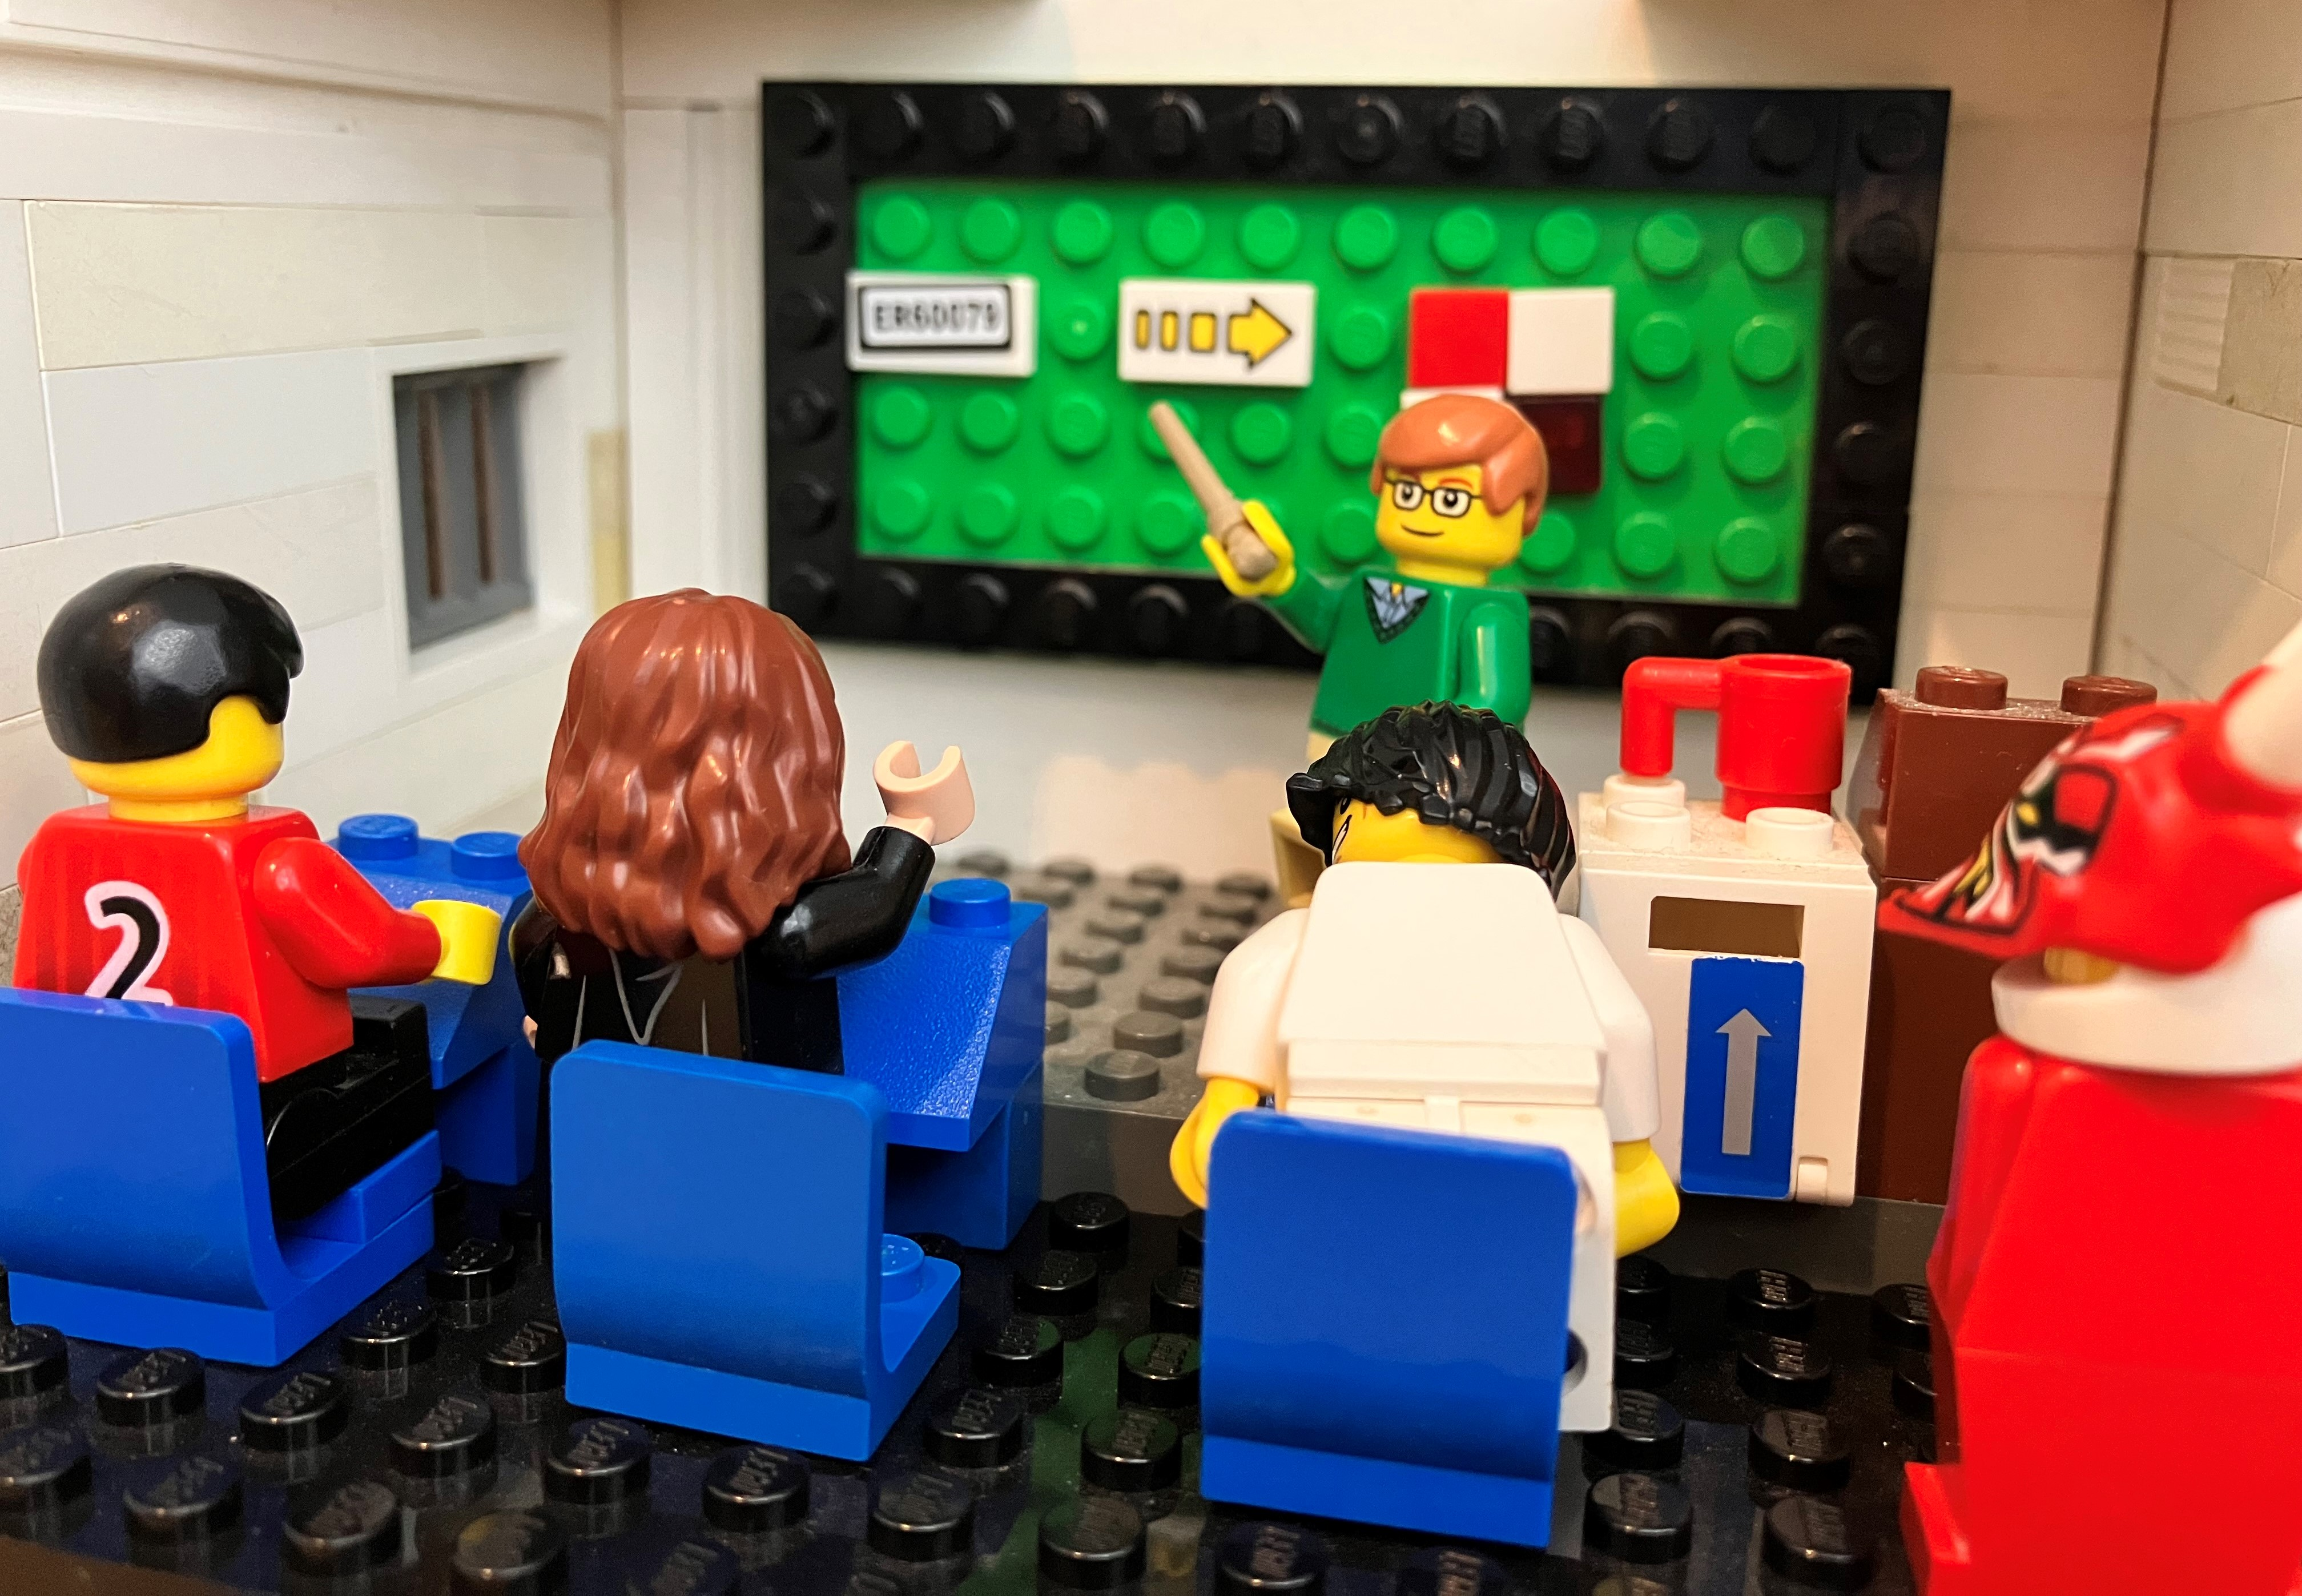
\includegraphics[width=4in]{front/motive.jpg}};
          \node at (0,3in) {
                \begin{tikzpicture}
                      \node[text width=3in,
                            fill=black!10,
                            cloud, 
                            cloud ignores aspect, 
                            minimum width=3in, 
                            minimum height=3in,
                            scale=1.25,
                            draw] at (0,2in) {That's right, this boring bit is really relevant today because it was on my qualifying exam...};
                      \node[text width=3in, scale=1] at (1in,1.5in) {...and on my advisor's exam...};
                      \node[text width=3in, scale=0.75] at (-0.5in,1.25in) {...and his advisor's exam...};
                      \node[text width=3in, scale=0.65,rotate=5] at (0.85in,1in) {...then Bernoulli---or was it his brother?!---homework find out which one...};
                      \node[text width=3in, scale=0.5,rotate=-7] at (-0.75in,0.85in) {...funny story, Archimedes...};
                                  
                \end{tikzpicture}};
    \end{tikzpicture}
\end{center}
\newpage



Algebra today is taught by example. First groups, then rings,
then fields, then modules, then bigger groups, then crazier non-associative
rings, then groups and rings with outside influences like topology, analysis,
and geometry. Today there are few general-practice algebraist.  There are
instead geometric group theorist, algebraic geometers, commutative ring
theorist, representation theorist, non-associative algebraist, computational
algebraist (that's me), and even those topics are too general for any one
theorist to master. Its acceptable because we still know one another and can ask
a specialist when we do not understand. 

The problem is that our algebra textbooks are getting thicker, some split into
multiple volumes. We have not covered an entire text for decades and few  
students can familiarize themselves with the entire book in one year.
One outcome has been to emphasize the good-old-days of successful theory from the
1800's and early 1900's.  Sylow's theorems, Wedderburn-Artin, Hilbert's
Nullstallensatz, Krull-Schmidt, Jordan-H\"older, Frobenius reciprocity. But a
lot a has happened in the century since.  Another approach has been for teachers to
pick their favorites making each course different form the next.  
Too many of us follow trends and fashions for this to be reliable (rebellion of 
a trends is a trend in its own right).

What if algebra were not taught by examples?  What if we taught its
underlying structural methodology and saw examples as reinforcing the theory
not being the theory.  What if instead of proving Krull-Schmidt for modules and
saying ``the same idea applies for groups and rings'', we just proved a theorem
that applied to modules, groups, and rings?  There is no harm in repetition and
useful examples.  I understand why we skip details of homomorphisms of modules
or Lie algebras because by the time students see these, they have seen enough
examples of that concept.  Yet, that behavior goes very wrong very quick.  Ask
your students (ask yourself) What is the kernel of a homomorphism of semigroups?
Monoids?  Homomorphism on $\mathbb{N}$?  Basic as these are, experience 
with groups and rings will not answer these riddles.
When we use our models instead of our theory 
we loose something.  

\begin{center}
    \textbf{Abstract algebra is not abstract enough.}
\end{center}


% \include{front/preface}
% \input{front/timeline}
\cleardoublepage


\tableofcontents
\cleardoublepage

% \input{front/notation}
\cleardoublepage


\mainmatter%%%%%%%%%%%%%%%%%%%%%%%%%%%%%%%%%%%%%%%%%%%%%%%%%%%%%%%


\import{1-intro}{index}


\part{Operators}
\cleardoublepage
\pagestyle{empty}
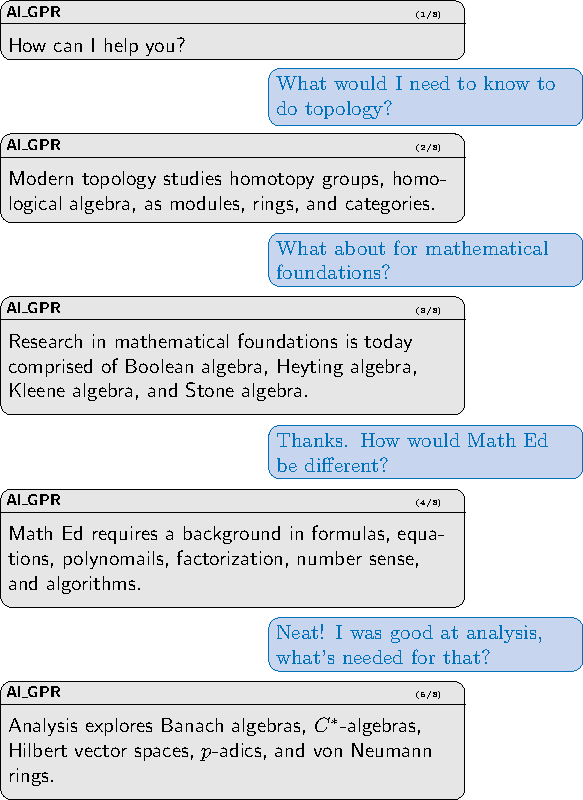
\includegraphics[width=\textwidth]{3-operators/AlGPR.pdf}
\newpage
\pagestyle{empty}
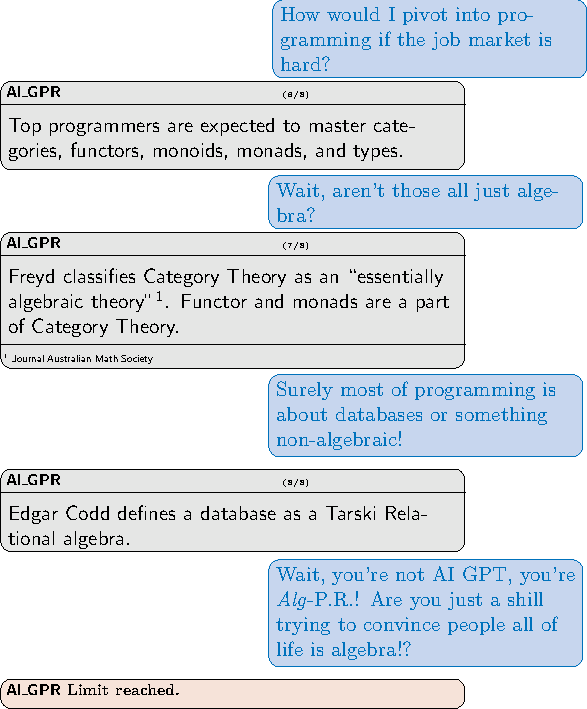
\includegraphics[width=\textwidth]{3-operators/AlGPR2.pdf}

\import{2-basic-ops}{index}
\import{3-operators}{index}

\import{4-lambda}{index}


\part{Equations with Variables}

\import{2-grammar}{index}

\part{Algebra}
\import{5-noether}{index}


\newpage
{\huge Answers...}
\begin{itemize}
      \item[$\Box$] What is an equation? A pair of formulas form the same unambiguous context-free grammar.
      \begin{itemize}
          \item[$\Box$] What is a context-free grammar? A model for expressing complex induction.
  
          \item[$\Box$] What is a variable? An element of the variable alphabet.
  
          \item[$\Box$] What makes an operator-variable? 
          A production rule in a context-free grammar set up as the signature of the formula.
  
          \item[$\Box$] What is a formula? A parse-tree of a context-free grammar with variables.

          
      %     \item[$\Box$] What is equality? (A variable with the Leibniz law as elimination.)
  
      \end{itemize}
\end{itemize}
{\huge Questions...}
\begin{itemize}
      \item[$\Box$] What is an algebra? (A collection of types and operators matched to the 
      production rules of a context-free grammar.)
      \begin{itemize}
          \item[$\Box$] What substitutes for an operator in a formula? 
          (A $\lambda$ which can be typed to match the production rules of the grammar.)
  
          \item[$\Box$] What substitutes for a variable in a formula?
          (Terms of of the types matched to the grammar.)
          
          \item[$\Box$] What substitutes for equality in a formula? 
          (A congruence on the algebra.)
      \end{itemize} 
      
  \end{itemize}





\import{4-algebras}{index}

% \import{6-free}{index}

% \part{Unassigned}
% \import{unassigned}{index}
% \chapter{What is algebra?}

Algebra is the study of equations, for the most part equations involving variables.
That is because applications have unknowns and if the
the shape of the equation can tell us anything about the 
options to solve it we shall want to take advantage of this.
Witness how we divide $ax^2+bx+c=0$ into solutions that are 
real or complex based on $b^2-4ac\geq 0$.  This is infinite variation 
in equations captured by strategy that divides into just 2 cases.

You probably already know every color, shape, and pattern of 
equation you will ever need.  Compare these two equations
\begin{align*}
    x^2+y^2 & \equiv 0 \pmod{541} 
    & 
    \frac{\partial^2 f}{\partial x^2}+\frac{\partial^2 f}{\partial y^2} & =0.
\end{align*}
These equations concern entirely unrelated contexts, for example $0$ on the
right is a whole number, whereas $0$ on the left is the function $0(x,y)=0.0$
Yet, the similarities as equations shine through.  This is because $0$, 
$+$, and  powers of $2$ are abstractions.  This doesn't connect them to
polarizing art movements nor render the concept inapplicable.  Abstract here,
and everywhere, means to study by limited attributes, which happens everywhere
in math and science.  So when we abstract the equation on the left we forget
about mod 541 and the precise meaning of these numbers.  On the right we forget
about functions and the notions of derivatives.  We are left with just $0$, 
$+$, and squares and where they sit, we abstract both to a common equation
\[
    x^2+y^2=0.
\]
In fact, even the equality was an abstraction which could vary from context to context.
With such flexibility a small number of symbols and their grammar are enough to capture 
the huge variety of equations we encounter in real life.

Now since every symbol in an equation is a variable we have new powers 
to solve equations.  Look to the humble 
\[
    x^2+1=0.
\]
By our own view, right now this is nothing but variables, so it means nothing to
solve this.  But, drop this into a context such as decimal numbers $\mathbb{R}$
and the understanding is to replace $1\defeq 1.0$, $0\defeq 0.0$, $+$ is
substituted for addition of decimals, and square is by multiplying decimals.
Equality now means two equal decimals, or in practice two decimal numbers that are close enough 
to be considered equal.  The only remaining unknown is $x$, but as everyone 
knows, we wont find a solution as no square decimal is -1.

The power of variable everything is that we are not stuck with the real numbers.
Lets replace everything with complex numbers $\mathbb{C}$. Substitute $0\defeq
0+0i$, $1=1+0i$, $(a+bi)+(c+di)\defeq (a+b)+(c+d)i$, and
$(a+bi)^2=(a^2-b^2)+2abi$.  Now we find $\pm i$ are the solutions. Solutions do
exist!  Since they exist we can return to a problem and ask if the solutions we 
found will do the job.  Maybe not.  

Why stop here? Try quaternions, or $(2\times 2)$-matrices.  These each have
addition, 0 and squares.  Now we learn there can be infinitely many solutions to
that equation.  If complex solutions were not right perhaps one of these
infinitely many quaternions or matrices will do.  This is the method of algebra:
find all the values that can be substituted into an equation to see what makes
solutions possible and how they behave.  Learn enough by this process and we can
begin to predict if solutions are to be expected and fathom algorithms to find
them when they do exist. When the solutions become infinite we find ways to
parameterize them with smaller data such as a basis.

Don't forget equality is variable too!  Suppose we wanted to solve $x^{541}+x+1=0$
using only integers.  Replace equality 
with $\equiv$ modulo 2 and ask for a whole number $x$ that solves
\begin{align*}
    x^{541}+x+1\equiv 0\pmod{2}.
\end{align*}
All integers in this equality become either $0$ or $1$, but neither will solve 
this equation.  By varying equality we confirm there are no solutions.


\begin{quote}
    \textbf{The power of algebra is that every symbol 
    in an equation is a variable, especially the equals sign.}
\end{quote}

% 
\section{Induction Operators.}
The rules in the grammar are often described as \emph{operators}.  For example,
\lstinline{<PosDig><Nat>} operates to take a positive digit and a natural number 
and form a new natural number.  We call it a \emph{binary} operator because it 
takes two inputs.  We also call it \emph{heterogeneous} because it takes in data 
of different types.  (If all the inputs and outputs are of the same type we call the operator 
\emph{homogeneous}.)  Some operators take in only one input, so-called \emph{unary},
such as squaring a number, or the first case of \lstinline{<Nat>} which takes in a digit and is said to \emph{promote} the 
term to a natural number.\footnote{Promote improves over the alternative \emph{coerce},
which in turn replaced the use of ``caste''---an all too casual allusions to a discriminator societal 
system.}
Operators that require no preexisting data, such 
as the digits $0,\ldots,9$, are called \emph{nullary}, or simply \emph{atomic}.

Each operator is an allowed step in an induction.  If it branches then two or more 
previously built items must be combined.  The atoms are what we call base-cases 
in the induction parlance.  The role of grammar on induction becomes all the more 
pronounced when we begin to give them distinguished roles.


\section*{Multi-sorted grammars.} To add depth to language we sort the allowed operators.  
The first sort are constants (aka the atoms or nullary operators).  The next sort are variables, e.g.\
$x,y,x_0,x_1,\ldots$. A third sort can be operators, e.g.\ $+,-,\times,\div$.
Symbols like parenthesis, braces and other groupings are usually considered as part of 
the meta-language and used to clarify how to read formulae, but not specifically part of any formula.
Like ``set'', ``sort'' now has this technical meaning.

\index{boolean algebra|(}
To make things short lets drop down to the language of Boolean (true/false) algebra.
\medskip

\noindent\textbf{Example.}
For Boolean (true/false) algebra we have true `$\top$', false `$\bot$', 
and `$\wedge$', or `$\vee$', and not `$\neg$' with the following grammar
which includes parenthesis. For example, $\top \vee (\neg(x_2\wedge y)\vee x_1):Bool$ but $Bool$ rejects $\bot\neg$.
\begin{lstfloat}[!hbtp]
\begin{lstlisting}[mathescape]
    <Var>  ::= x | y | x_<Nat> | y_<Nat>
    <Bool> ::= $\top$ 
             | $\bot$ 
             | <Var>
             | $\neg$ <Bool> 
             | <Bool> $\vee$ <Bool> 
             | <Bool> $\wedge$ <Bool>
             | (<Bool>)
\end{lstlisting}
\caption{A Boolean algebra grammar.}
\end{lstfloat}

There is something still missing.  Try reading $\neg(x_2\wedge y)\vee x_1$.  
Is this meant to negate $(x_2\wedge y)\vee x_1$ 
or is it to negate $(x_2\wedge y)$ and then or that with $x_1$? This grammar 
offers two associated parse trees.
\begin{center}
    \begin{tikzpicture}
        \node at (-3.5,0) {\begin{tikzpicture}
            \node (10) at (0,0) {$\neg(x_2\wedge y)\vee x_1:Bool$};
            \node (0n) at ( 0,-2) {$(x_2\wedge y)\vee x_1:Bool$};
            % \node (0d) at ( 2,-4) {0:Digit};
            \draw[thick] (0n) -- (10);
            % \node[below of=10,scale=0.75] {$\circ$};
            \node at (0.5,-1) {$\neg$};
            % \node[scale=0.75,text width=0.6in] at ( 1.5,-3) {Nat case 1};
        \end{tikzpicture}};
        \node at (3.5,0) {\begin{tikzpicture}
            \node (01) at (0,0) {$\neg(x_2\wedge y)\vee x_1:Bool$};
            \node (1) at (-2,-2) {$\neg(x_2\wedge y):Bool$};
            \node (0n) at ( 2,-2) {$x_1:Bool$};
            \draw[thick] (0n) -- (10) -- (1);
            \node[below of=01] {$\vee$};
        \end{tikzpicture}};
    \end{tikzpicture}
\end{center}
\index{first order logic}
What we have built is very nearly the \emph{free boolean algebra of countable rank}, or 
sometimes known as 1st order logic. The missing ingredient (relations) will come later.
It is demonstration of how a lot of algebra can be built.  You start with some desired 
operators, some constants, and some variables and you build it by induction.
\index{boolean algebra|)}
\section{Order of operations.}
\emph{Order of operations} steps in to resolve the ambiguity.
One option is \emph{left-most outer-most (LeMOM)}, which---similar to English language,
reads from left to right and assumes we start to match the pattern from the 
outer most symbols.  So  $\neg(x_2\wedge y)\vee x_1$ in LeMOM means
$\neg$ is the symbol we need to parse first.  That requires us to 
build a \lstinline{<Bool>}.  So we move left and read 
$(x_2\wedge y)\vee x_1$.  Here the LeMOM is `(' which will need to match 
with \lstinline{<Bool>)}.  Reading further $x_2:Var$ which promotes to 
$x_2:Bool$, but this is not followed by `)' so it must continue left-ward.
Next is $\wedge$ which matches with $x_2:Bool\wedge y:Bool$
so that we have $x_2\wedge y:Bool$.  Then we hit `)' which matches 
our earlier `('.  Now we finally get $(x_2\vee y):Bool$ which finally matches with 
$\neg$\lstinline{<Bool>}.  We have parsed $\neg(x_2\wedge y):Bool$.  At this point 
we have parsed $\neg$ and so we continue with $\vee$ to match 
$\neg(x_2\wedge y)\vee x_1:Bool$ with the right-hand-side parse tree.


LeMOM parsing is favored in mathematics and computer science because we can 
decide what things mean the moment we encounter them in the string.  
There are other orders of operations,
for example right-most inner-most (RiMIM) or the high-school PEMDAS
(Parenthesis, Exponential, Multiplication, Division, Addition, Subtraction). 
These allow for short formulas to be more expressive (jargon to mean they 
communicate more than a similarly long string in a less ``expressive'' language).

\begin{quote}
\textbf{Grammar plus order of operations are a language to express an induction.}
\end{quote}

\noindent\textbf{Exercises}
\begin{enumerate}
    \item Write the grammar for decimal numbers.
    \item Write the grammar for a 4 function calculator with decimal numbers
    and $+,-,\times, \div$.
\end{enumerate}
\medskip

% \subsection{Operators that generate}
Incrementing is more a definition than it is a 
 case of adding 1.
A natural number is either $0$, or a successor 
$S(k)$ to 
another natural number $k$.  Often this is expressed as a 
definition where $\mid$ stands for separating cases, 
for example:
\begin{align*}
    \mathbb{N} \defeq 0 \mid S(k)
\end{align*}
So $0$ is ``zero'', and $1$ is just a symbol representing $S(0)$, 
$2\defeq S(S(0))$ and so on.  Replace $S$'s with tally marks (not to be 
confused with `$|$' used as an ``or'' above)
we recover childhood counting:
\begin{center}
    $0\defeq$ \underline{\hspace{5mm}}, 
    $1\defeq$ \StrokeOne,
    $2\defeq$ \StrokeTwo,
    $3\defeq$ \StrokeThree,
    $4\defeq$ \StrokeFour,
    $5\defeq$ \StrokeFive,...
\end{center}
The point is, the successors are not so much a function 
moving around the numbers we have, it actually is a producer 
of numbers. 

Perhaps because it is so primitive, this is an idea we 
can imitate to create more meaningful values, like a string 
of characters in an alphabet \lstinline{Char:=['a','b',...,'z']}.
\begin{lstlisting}[language=Hidris]
data String = Empty | Prepend( head:Char, tail:String) 
\end{lstlisting}
Writing \lstinline{head:Char} or \lstinline{tail:String} 
indicates that head must come from the alphabet we chose 
and tail must be some already produced string, possibly empty.
Some readers might relate to a different dialect of 
programming such as the following
\begin{lstlisting}[language=Sava]
class String
    case Empty extends String
    case Prepend( head:Char, tail:String) extends String
\end{lstlisting}
The head here caries around what we put in the list and the tail 
is what comes next in the list.  Observe the similarities:
\begin{align}
     2 & \defeq S(S(0)) \tag{$\mathbb{N}$}\\
 \text{\lstinline{"me"}} & \defeq \text{\lstinline{Prepend('m',Prepend('e',Empty))}}
\tag{String}
\end{align}
The left-hand sides are merely notation for what the data really is on the right.
Both the successor and the \lstinline{Prepend} are operators that generate 
new values.  So part of algebra is to generate new data; so, it is no wonder 
that it closely connections to computation.

\subsection*{Exercise}
\begin{enumerate}
    \item Mimic the String data type to make a list of integers (that is 
    switch from the alphabet to integers).

    \index{generics}
    \item Mimic the String data type to make a list of fixed by 
    unknown data of type $A$, call it \lstinline{List[A]}.\footnote{
    Alternatives include \lstinline{List a} and \lstinline{List<A>}. 
    Search for \emph{generics} in your programming language to learn more.
    }

\end{enumerate}
\index{nil}\index{cons}\index{list}
Historically \lstinline{Empty} for lists is called \lstinline{Nil} 
and \lstinline{Prepend} is called \lstinline{Cons}.

\subsection{Generated operators}
We can take this the idea of generating further, for example, using 
the unary operator, successor, prepend, etc., and have them generate 
binary operators.
\begin{align*}
    m+n & \defeq\left\{ 
    \begin{array}{ll}
        n & m = 0\\
        S(n+k) & m=S(k)
    \end{array}
    \right.
\end{align*}
So does $2+4=6$?  We can test this out.
\begin{align*}
    \text{\StrokeTwo}+\text{\StrokeFour} & = \text{\StrokeOne}~ \big(\text{\StrokeOne} +\text{\StrokeFour}\big)\\
    & = \text{\StrokeOne}~ \big( \text{\StrokeOne}~\big(\underline{\hspace{5mm}}+\StrokeFour\big)\big)\\
    & = \text{\StrokeOne}~ \big( \text{\StrokeOne}~\StrokeFour\big)\\
    & = \text{\StrokeOne}~ \text{\StrokeFive}.
\end{align*}
Try this for strings
\begin{align*}
    s+t & \defeq\left\{ 
    \begin{array}{ll}
        s & t = \texttt{Empty}\\
        \texttt{Prepend}(x,s+tail) & t=\texttt{Prepend}(x,tail)
    \end{array}
    \right.
\end{align*}
What is \lstinline{"awe"+"some"}?  

While no one will seriously add integers as a tally, 
knowing that it can be done establishes a pattern which can be exported to other context
with meaningful new structure.  Just notice $3+4=4+3$ but not so with adding strings.
These siblings have their own personalities, and it this might even help us recognize 
that while $3+4$ does equal $4+3$ it might be for somewhat subtle reasons.

What about multiplication? Isn't is just this:
\begin{align*}
    m\cdot n\defeq \overbrace{n+\cdots +n}^m.
\end{align*}
That is nice, but seems to leave us to figure out missing parenthesis or set aside 
time to prove they don't matter.  I am in the mood to continue making things rather 
than study them.  Lets repeat what we have done.
\begin{align*}
    m\cdot n & \defeq \left\{
        \begin{array}{ll}
            0 & m=0\\
            k\cdot n+n & m=S(k).
        \end{array}
    \right.
\end{align*}
It works, but check it out for yourself.  And for strings what might we get?
\begin{align*}
    s\cdot t & \defeq \left\{
        \begin{array}{ll}
            0 & s=\texttt{Empty}\\
            \texttt{Prepend}(x,k\cdot n)+n & s=\texttt{Prepend}(x,tail)
        \end{array}
    \right.
\end{align*}
What is "Mua"$\cdot$"Ha"?
%% Mua*Ha=MuaHaHaHa
You can carry on to make exponents and more.  If you do you may find 
Knuth arrow notation helpful on your journey, look it up.


\subsection{Operators measuring defects}
Algebraist spend a lot of time worried about misbehaving operators 
causing them to generate new operators that spot the flaws.  This is another 
source of higher valence operators. If 
we can add, subtract, and multiply then we can make the following operators as well.
\begin{align*}
    [a,b] & = ab-ba \tag{Commutator}\\
    (a,b,c) & = a(bc)-(ab)c \tag{Associator}
\end{align*}
Commutative algebra requires $[a,b]=0$ while associative algebra needs $(a,b,c)=0$.
For example matrices fail to be commutative algebra but are associative.
Replace the role of multiplication of matrices with $[a,b]$ and ask for it's 
associate, i.e.
\begin{align*}
    (a,b,c)_{[,]} & = [a,[b,c]]-[[a,b],c]
\end{align*}
and we no longer get associative nor commutative algebra.  These are structures 
known as Lie algebras.  While not associative, because they are based originally 
on matrix products that are associative we can stumble eventually upon a 
graceful alternative
\begin{align*}
    0 & = [a,a] \tag{Alternating}\\
    0 & = [a,[b,c]]+[b,[c,a]]+[c,[a,b]].    
    \tag{Jacobi}
\end{align*}
So the problem is not getting worse, at least we wont be needing 
to look into some  valence 4 operators as defects.  Sabinin algebra 
studies how defects in operators pile up or die off.



Keep in mind requiring that $[a,b]=0$ or $(a,b,c)=0$ is an equation. 
Like any equation it has limited solutions.  By that reasoning, 
most of algebra wont behave commutative nor associative.




% 
\section{Paradox of the Trapped Variable.}
Think back to substitution in $x(x+3)^c$.  Suppose we use 
the rules to substitute $c\defeq 2$, we get $x(x+3)^2$, $c\defeq \pi$ gives 
use $x(x+3)^{\pi}$.  For $c\defeq d$, we want $x(x+3)^d$.  
Now try $c\defeq x$.  Would you really 
convert this to the function $x(x+3)^x$?  Maybe, but it is more likely that 
we see $x$ and $c$ as distinct, that is, $c$ is constant to $x$.
Something about substitution does not follow induction as cleanly as we have described so far.
If you don't see this as a problem yet lets look at something more basic.

Lets slow down to see what happened.  Set:
\begin{align*}
    I(x) & = x & 
    K_c(x) & = c.
\end{align*}
You may call $I$ the identity function and the $K$ constant functions.
% but with excessive mathematical training you are likely to overthink 
% the situation.  These two formulas have no use for domains and codomains for 
% instance.  We can safely use these even when there are no sets or mathematics 
% around to make sense of deeper concepts.
Try some substitutions, I tried $I(3)=3$, $I(\clubsuit)=\clubsuit$.
I found $K_3(2)=3$ and $K_3(\clubsuit)=3$ as well.  I even tried 
$K_{\clubsuit}(2)$ and got $\clubsuit$.  I changed $x$ for $y$, 
$I(y)=y$, and $d$ for $c$, $K_d(x)=d$. Next I substituted $x$ for $c$ and got
\begin{align*}
    K_x(x)=x=I(x).
\end{align*}
Now we have a true problem: a constant function should not equal 
an identity function.\footnote{Functions in this sense are so primitive 
they have no domains and codomains.  You can put anything into these functions.}
This is the paradox of the trapped variable.

As my philosophy  colleague Professor Dustin Tucker says, 
``A system studied long enough reveals its paradoxes.'' 
Paradoxes (para = distinct + dox = opinion) are inconsistencies that you can avoid by revisiting the scope 
of your definitions.  Just withhold some options and you wont end up with 
two different options.  It is not a philosophically satisfying resolution,
which is why most paradox hacks lead to schisms. 

So what is the root cause of our paradox of the trapped variable?
The answer are bound (local) verses free variables. 

To avoid trapped variables I use the rules set out by Curry-Feys.
First you need a grammar.  Keeping to context free and learning by example

Why did something so basic fail?  It has to do with variables coming in 
two forms: free and bound.  If you program you might think of a global 
verses local variable.  First things first: variables?
First sort out the data.  One sort will be constants, atoms like an alphabet,
maybe digits, or a word or special symbol. A second sort will be called variables.
That its, variables are symbols from special alphabet we call variables.
This means that a variable can never equal a constant, statements like $x=2$ 
are in strict sense nonsense.  But hold off on that journey for a moment.
Now having all these alphabets we can form strings using the various letters.
We could define arithmetic using digits $0,\ldots, 9$, $+,-,\times,\div$ and some 
variables but lets simplify things to true/false which is long enough to 
explore the idea.  We need to specify a grammar of how allowed formulas can 
be made.  We basically separate the options by $\mid$ (reads as ``or'')
and use patterns to explain structures that are built up recursively.
So for Boolean (true/false) algebra we have true $\top$, false $\bot$, 
and $\wedge$, or $\vee$, and not $\neg$ language might be defined like this.
\newpage    
\begin{lstfloat}
\begin{lstlisting}[mathescape]
    <var>  ::= x | x_<int>
    <Bool> ::= $\top$ 
             | $\bot$ 
             | <var>
             | $\neg$ <Bool> 
             | <Bool> $\vee$ <Bool> 
             | <Bool> $\wedge$ <Bool>.
\end{lstlisting}
\end{lstfloat}

To get started lets return to our use of a grammar.  The diagram we had 
was a tree, what is known as a \emph{parse tree}.  It is the same thing you 
do when you diagram a sentence in grammar school, only with English you can 
sometimes get cycles.  That we got a tree is owed to the fact that the grammars 
for mathematics are basic and gentle, what Chompsky calls \emph{context-free} grammars.

This situation comes about because of two flavors of variables: free and bound,
also called local.  A variable can be bound in many ways, for example 
$\forall x$ binds $x$ to $\forall$, same with $\exists x$.  The binding tells 
us that even if we are using $x$ somewhere else, form this point till 
the end of the block we are simply recycling the name $x$, but its meaning 
is now controlled by the start of the binding.  The binding in the 
substitution examples above is hidden by notation but it is third form 
known as $\lambda$-binding, such as $x\mapsto x+2$ (historically 
$\lambda x.(x+2)$ which is where the name comes from).  This says that 
$x$'s role is to serve as the variable in describing a function.
In the constant function $c\mapsto K_c$ or rather $c\mapsto (x\mapsto c)$.
Likewise $\sqrt{n}{u}$ means $n\mapsto (u\mapsto \sqrt[n]{u})$
Now the point is that a local variable is just reusing a symbol it has 
no visibility outside.

Why did something so basic fail?  It has to do with variables coming in 
two forms: free and bound.  If you program you might think of a global 
verses local variable.  First things first: variables?
First sort out the data.  One sort will be constants, atoms like an alphabet,
maybe digits, or a word or special symbol. A second sort will be called variables.
That its, variables are symbols from special alphabet we call variables.
This means that a variable can never equal a constant, statements like $x=2$ 
are in strict sense nonsense.  But hold off on that journey for a moment.
Now having all these alphabets we can form strings using the various letters.
We could define arithmetic using digits $0,\ldots, 9$, $+,-,\times,\div$ and some 
variables but lets simplify things to true/false which is long enough to 
explore the idea.  We need to specify a grammar of how allowed formulas can 
be made.  We basically separate the options by $\mid$ (reads as ``or'')
and use patterns to explain structures that are built up recursively.
So for Boolean (true/false) algebra we have true $\top$, false $\bot$, 
and $\wedge$, or $\vee$, and not $\neg$ language might be defined like this.
\newpage    
\begin{lstfloat}
\begin{lstlisting}[mathescape]
    <var>  ::= x | x_<int>
    <Bool> ::= $\top$ 
             | $\bot$ 
             | <var>
             | $\neg$ <Bool> 
             | <Bool> $\vee$ <Bool> 
             | <Bool> $\wedge$ <Bool>.
\end{lstlisting}
\end{lstfloat}




Before leaving a word on \emph{sorts}.
Refine this as you like. For instance, one sort $a,b,c,\ldots,m,n,\dots, x,y,z,
x_1,x_2,\ldots$ for numbers, a sort $+,-,\times, [\ldots]_{\ell},\ldots$ for
operators, $\cong, \equiv, \ldots$ for equality.  You decide, it is a made up 
language.



  Formulas are strings over these alphabets.  Each of these has a 
a grammar and a handy notation is 
to separate options by $\mid$ which reads as \emph{or}.  For example, 
a true $\top$, false $\bot$, and $\wedge$, or $\vee$, and not $\neg$ language might be defined like this.
\newpage    
\begin{lstfloat}
\begin{lstlisting}[mathescape]
    <var>  ::= x | x_<int>
    <Bool> ::= $\top$ 
            | $\bot$ 
            | <var>
            | $\neg$ <Bool> 
            | <Bool> $\vee$ <Bool> 
            | <Bool> $\wedge$ <Bool>.
\end{lstlisting}
\end{lstfloat}

So $x$ is a boolean, as is $\top$ and $\neg x\wedge x_3$.  Math languages assume 
also the symbols for parenthesis.

of variables for numbers will be $m,n,\ldots,
x,y,\ldots$ whereas a separate sort of variable is used for operations, such as
$+,-,\times,\ldots$, and still another $A,B,C,\ldots$ for sets and so forth.
Sorts used in this way have formal meaning in logic and I mention that because 
you will come across it in examples of formal methods---the growing field 
blending the idea of proving theorems with proving programs, what we will 
need to make safe self-driving cars and video games that you can't cheat.

Starting with a string $M$ with symbols of various sorts, the task is to 
substitution variable $x$ in by another string $N$.  If there is only one 
variable around you may think of this as $M(N)$.   Since $M$ may have many 
variables let us be specific:
\begin{align*}
    M[x\defeq N]
\end{align*}
To see how to do this lets break the down th process of making $M$.
For example we might be in context of a simple calculator.  So our constants 
are the digits $0,1,\ldots,9$, and we have also $+,-,\times,\div$.
Variables we call $x,y,z$ and if we need more $x_n$ where is a sequence 
of digits will do.


We can start out small with two sorts of data.  One 
sort are atomic symbols, digits, an alphabet or some other meaning 
of a constant.  The second sort are variables.  Then we formula 
$M$ is either an atom $a$, a variable $x$, or the concatenation 
of two formulas $K$ and $L$.  There is a popular notation for this 
is to separate each case by the stroke $\mid$ which reads as ``or''.
\begin{lstlisting}[language=Hidris,mathescape]
    F[X] = 0 | 1 | ... | 9 | + | -
         | x
         | <F[X]> cat <F[X]>
\end{lstlisting}

So if our atoms are $\clubsuit,\heartsuit, \spadesuit,\diamondsuit$
and 
\begin{lstlisting}[language=Hidris,mathescape]
    F[X] = a:A 
         | x:X
         | K:F[X] cat L:F[X]
\end{lstlisting}

\begin{lstlisting}[language=Hidris,mathescape]

    M[x:=N] =
        match M with 
                a:A $\Rightarrow$ a
                y:X $\Rightarrow$ if x=y then N else y
            K cat L $\Rightarrow$ K[x:=N] cat L[x:=N]
             y $\mapsto$ L $\Rightarrow$ if x=y then y $\mapsto$ L 
                                         else if x free in L 
    \end{lstlisting}
    

\begin{lstlisting}[language=Sava,mathescape]
F[X] = a:A 
     | x:X
     | M:F[X] cat N:F[X]
     | x:X $\mapsto$ M:F[X]

M[x:=N] =
    match M with 
            a:A $\Rightarrow$ a
            y:X $\Rightarrow$ if x=y then N else y
        K cat L $\Rightarrow$ K[x:=N] cat L[x:=N]
         y $\mapsto$ L $\Rightarrow$ if x=y then y $\mapsto$ L 
                                     else if x free in L 
\end{lstlisting}




% 
\chapter{Free algebra}


% \chapter{Types of algebra}

You can add music, well at least you can play two songs at the same time.
Is that again music?  Probably it is safer to say we can add sound, and 
some sound is music.  This is thinking like an algebraist.  This is 
clarifying that addition has a context.  Operations are carried out 
without leaving that context.  We say that:
\begin{quote}
    ``Sound is closed under addition.''
\end{quote}
You needn't be too strict about the context.
When you add a list of length 3 to a 
list of length 3 it gets to a list of length 6, not 3.
Just like music is to sound, a list of length 3 is to a list of any length.
We recover closure by adding lists of all sizes.

Broadening our context may not be enough.  When we divide 
we avoid division by $0$.  When we subtract natural numbers $m-n$
we need $m\geq n$.  When we compose functions we need the 
domain of the second to contain the image of the first.
You might be in a place to fix this, for example add $\pm\infty$ 
to define as $x/0$ or negative numbers to account for $3-5$.
Functions $f$ and $g$ that cannot be compose can be composed as relations:
\begin{align*}
    (g\circledcirc f)(x) \defeq \{z\mid \exists y, y=f(x), z=g(y)\}.
\end{align*}
When doing algebra with such operators we nearly always spend 
our time explore independent cases, most of which are 
roughly speaking ``errors''.  The better idea is to acknowledge 
we don't really want to divide by 0, produce negatives we are not using,
or composing non-composable functions.  It is time for types.



What to do isAny system 
A paradox is not a contradiction


Evidently $I(2)=2$ and $K_3(2)=3$.  These definitions are so simplicistic 
they work without a domain or co
The function on the left is an identity function, changing nothing 
to the given inputs.  The functions on the left are constant functions, 
ignore the input and outputing a fixed value.  Neither concept 
is in need of a domain or domain, which is convenient when explaining 
functions before there are sets, such as when we program, or when sets 
aren't big enough, such as trying to make a set of all sets.

Using what we know about substitution we can choose the constant $c$
however we want, maybe 2, maybe $\clubsuit$, or another variable $y$.
So why not substitute $x$ for $c$?
\begin{align*}
    K_c(x)|_{c\defeq x} & = x = I(x).
\end{align*}
A constant function is suddenly the identity function, which cannot be 
right.  This is a mistake in substitution known as the \emph{paradox of 
the trapped variable} and what it tells us that substitution is not so 
naive after all.

We call the first an \emph{identity} function and the second is a \emph{constant}
function.  This notation is misleading, technically $I$ is a symbol
which denotes some unknown process such that when applied to data $\clubsuit$,
its output, often denoted $I(\clubsuit)$, is given input data unchanged.
So $I(\clubsuit)=\clubsuit$ is a judgement we can make about an identity 
function not a program.

There is a bit of implicit information in our use 
of parenthesis and what they mean.  Traditionally $I$ and $K$ are 
the functions.  An input $\clubsuit$ passed to a function $I$ 
yields an output denoted $I(\clubsuit)$.  In the case of the identity 
function $I$ does nothing to modify the input so we can judge 
$I(\clubsuit)=\clubsuit$.  Since this applies for any input we 
can abstract over the inputs by replacing their role with a variable 
$x$ and write $I(x)=x$  It is not a definition of $I$ so much as 
a consequence.  Of course we could use the outcome rule to conjure 
a perspective algorithm to perform the function.  When we do this 
we often insert some extra language like ``define I(x)=x'' or 
use the Walrus notation $I(x)\defeq x$.  In programs words like 
define are abbreviated.  For example, the following two programs satisfy
the identity function rule without following the same process.
\begin{lstlisting}
    def doNothing(x) = x 
    def doNothingUseful(x) = compute 200! then return x
\end{lstlisting}
Much of the feasibility of algebra comes down to appreciating 
different processes that achieve the same overall calculations.


Suppose we have two types of data, one we call $A$ and the other $B$.



\subsection{Operators forced into service}
Sometimes you have an operator and it doesn't work.
to be clever, even lucky, to guess at an operator.
In famous history, Heisenberg escaped to an island from Copenhagen 
to avoid hay-fever, or an over zealous host Niels Bohr. 
Able to think clearly he summarized what he knew: a particle $\psi$
could take possibly many states, maybe spin up $\uparrow$ or spin down 
$\downarrow$.  so it record this as linear combination
it as a linear combination $|\psi\rangle = \alpha|\uparrow\rangle+\beta|\downarrow\rangle$
where in vector space with $\{\uparrow,\downarrow\}$ as a basis. 


The Copenhagen interpretation suggested that the particles 
was in a mixture of states that when observed would spontaneously collapse 
to one of $\uparrow,\downarrow$.  Others think everything happens just in 
other universes but I don't see why the only normal universe would be 
randomly the one I am in so I think that notion is equaly philosophical and 
meaningless.  Perhaps quantum Bayssian interpretations make sense.  There is 
some unknown distribution of the particle, , 
The $\alpha$ and $\beta$ explained the probability that when we 
measure the state of $\psi$ 

somewhat famously 
was having difficulty with hay-fever in Copenhagen and was stuck with 
quantum puzzles who could not solve. Clearing his head on an island 
he conjured the view that particles $\psi$ could be viewed as linear 
combinations of all the states the could o
$\langle \psi|=\alpha \langle $ consisting of the probabilities of each state.
recognized matrices capture all the states of a quantum system and 
to compute the next event involv



\subsection{Further operators}




These examples lean on some addition pre-existing somewhere.  





\section*{Other operators}



To enforce a philosophy such as that some algebra is closed to 
operators 
Such a philosophy is one 


To get the details rolling in earnest we must know the application.
The world around us partly interacts with computers so lets assume 
this is a uniform assumption: any problem in algebra that I want to 
state should be expressible to a computer.  That computer might not 
be able to handle it but its hard to imagine an equation we need 
to consider where the equation itself cannot be stored in a computer.




That is one philosophy, a philosophy where addition is an abstraction.
That word makes some bristle.  It reminds them of polarizing art 
installations or refrains from the bar room rants between pure and 
applied thinkers.  Abstract, for for those who reason, means to limit 
argument to specified attributes.  Thats every type of math and a good 
chunk of science so it shouldn't raise dismay.  \emph{Raising the level of 
abstraction} is then just the declaration the we're about to gather the 
instance we have and ma

Perhaps you feel some one owes you a foundation for addition, 
a place you derive what addition really means before you 
take to making it show up everywhere else.
You can count on it, literally.
\begin{align*}
    \mathbb{N} & = 0 | S~k.
\end{align*}


\chapter{How do we do algebra?}

This leaves us with the job of making those data which can be substituted 
into equations.  This means firstly new numbers that, like the decimals, complex 
numbers, polynomials or matrices; can give a meaning to things like $0$ and $1$
and eventually the answers $x$ we seek in solving applications.  Secondly 
we need to find what works for the operations, the sums, squares, products, and 
etcetera.  Last and most important in the method of algebra is to invent the possible 
substitutes for equality, what algebraist call \emph{congruences}.  

Over 2 centuries the methods have evolved and with it notation and emphasis to
the point where the three roles just articulated may not be recognizable.  
This is where it becomes necessary to add in constraints: a family of problems 
you need solved that guide you to the algebra you need.  But when we pause to see 
the similarities we can carry forward a far great number of algebraic lessons 
than we can by concentrating only on the best tools for individual examples.
That will be our perspective.  To further constrain the study we invite in 
applications that constrain the questions to important families the ones
which might solve your problem or lead you to the algebra the may one day define you.


% \chapter{Formulas \& Equations}

Lets get precise about equations.  They have a left hand side and right hand side.
But the items that can occur on the left can also occur on the right so we could 
define any one side and be done.  The equations worth study are those involving 
variables, more precisely variable and operations since and equation $x\cdot y=1$ is 
infinitely more interesting than $x=1$.  So we start out with what are called 
formulas, but you would do well to think of these as generalized polynomials, 
only we might involve more operations than simply those found in common polynomials.
As a byproduct we will re-invent induction in a form that is used everywhere in 
in the design of software data types.  


\appendix



\backmatter%%%%%%%%%%%%%%%%%%%%%%%%%%%%%%%%%%%%%%%%%%%%%%%%%%%%%%%


\bibliographystyle{plain}
% \bibliography{bibliography/tensor_biblio}



\printindex

%%%%%%%%%%%%%%%%%%%%%%%%%%%%%%%%%%%%%%%%%%%%%%%%%%%%%%%%%%%%%%%%%%%%%%

\end{document}





